%% Springer Nature (sn-jnl) version for Rock Mechanics and Rock Engineering.
%% Compile on Overleaf with the "Springer Nature LaTeX Template" (sn-jnl.cls).
%% Build:  pdflatex -> bibtex -> pdflatex -> pdflatex
%% Upload alongside this file:  refs.bib  and a figures/ folder with all the
%% PNGs listed at the foot of this preamble.
%%
%% Reference style: sn-basic (Springer author-year, used by RMRE). To switch to
%% numbered references use [pdflatex,sn-mathphys-num] and \bibliographystyle is
%% then set by the class.
\documentclass[sn-basic]{sn-jnl}

\usepackage{graphicx}
\usepackage{amsmath,amssymb,amsfonts}
\usepackage{booktabs}
\usepackage{subcaption}
\usepackage{siunitx}
% siunitx v3 (Overleaf) removed \SI/\SIrange; provide them if absent.
\providecommand{\SI}[2]{\qty{#1}{#2}}
\providecommand{\SIrange}[3]{\qtyrange{#1}{#2}{#3}}
\providecommand{\diameter}{\ensuremath{\varnothing}}
\sisetup{detect-all}

\graphicspath{{figures/}}

\newcommand{\Cz}{C_{0}}
\newcommand{\eps}{\varepsilon}
\newcommand{\epsd}{\dot{\varepsilon}}

\begin{document}

\title[Monash True-Triaxial Hopkinson Bar and Computational Workspace]{Development of the
Monash True-Triaxial Hopkinson Bar System and an Integrated Computational Workspace for
Multiaxial Dynamic Rock Characterisation}

\author*[1]{\fnm{Qianbing} \sur{Zhang}}\email{qianbing.zhang@monash.edu}

\affil*[1]{\orgdiv{Department of Civil and Environmental Engineering},
\orgname{Monash University}, \orgaddress{\city{Clayton}, \state{VIC},
\postcode{3800}, \country{Australia}}}

\abstract{Conventional split-Hopkinson pressure bar (SHPB) testing characterises rock
under one-dimensional dynamic loading, yet rock in deep mining, tunnelling and
rock blasting fails under \emph{multiaxial} stress states at high strain rate.
This paper presents the development of the Monash triaxial Hopkinson bar
(Tri-HB) --- a gas-gun-driven system of three independent pairs of orthogonal
square bars with hydraulic confinement on all three axes, enabling true-triaxial
($\sigma_2\neq\sigma_3$) static--dynamic coupled loading --- and an integrated
\emph{computational workspace}, the Virtual Tri-HB, that unifies test design, three-wave
data reduction, stress-path interpretation and damage modelling in a single
six-step workflow. We report six advances embedded in the computational workspace: (i) a
unified treatment of uniaxial, axisymmetric-confined and true-triaxial
static--dynamic loading as special cases of a single gas-gun system, reduced
through a consistent per-axis three-wave analysis; (ii) a
true-triaxial, Lode-angle-dependent and rate-dependent failure envelope that
captures the intermediate principal stress effect with the correct sign; (iii) an
energy-consistent damage--dissipation partition in which the first law closes by
construction with non-negative dissipation,
$W_{\mathrm{input}}=W_{\mathrm{el}}+W_{\mathrm{diss}}$ ($W_{\mathrm{diss}}\ge0$);
(iv) an orthotropic damage tensor whose components are driven chiefly by the
directional tensile strain (with a small shear/compaction term), reproducing the
directional (axial-splitting) fracture of rock blasting with a modest, nonzero
axial damage; (v) a cumulative-damage model for repeated (cyclic) dynamic
loading that reproduces the sudden, few-impact ($N_f\!\lesssim\!10$)
dynamic-fatigue failure of a pre-stressed rock mass; and (vi) a spatial
thermodynamic extension comprising a gradient-regularised damage field (internal
length $\ell$ calibrated from CT crack spacing) and a phase-field formulation
(Griffith energy $G_c$ from the measured dissipation and CT fracture area,
phase-field $\phi(\mathbf{x})$ validated against CT attenuation maps) that is
thermodynamically consistent by construction and directly comparable to
post-impact CT cross-sections. Because the three orthogonal bars measure
direction-resolved stress, strain and wave speed, each component of the damage
tensor can in principle be calibrated independently --- a capability a uniaxial
SHPB cannot provide. We close with a calibrate-then-blind-predict validation
roadmap that positions the Tri-HB and its computational workspace for quantitative,
multiaxial dynamic constitutive modelling of rock.}

\keywords{triaxial Hopkinson bar, dynamic rock mechanics, true-triaxial loading, intermediate principal stress, anisotropic damage, rock blasting, computational workspace, gradient damage, phase-field fracture, CT calibration}

\maketitle

\section{Introduction}\label{sec:intro}

The dynamic mechanical response of rock governs the safety and efficiency of
deep underground excavation, rockburst mitigation and rock blasting, where
loading rates of $10^{1}$--$10^{3}\,\mathrm{s}^{-1}$ coincide with confining
stresses of tens to hundreds of megapascals~\citep{zhang2014,WANG2026106436}. Capturing
this response in the laboratory has driven more than a century of development of
the Hopkinson bar, yet the classical apparatus remains one-dimensional. This
section traces that development, examines how confinement has conventionally been
added, and motivates a true-triaxial alternative.

\subsection{From the Hopkinson bar to the split-Hopkinson pressure bar}

The technique originates with Bertram Hopkinson, who in 1914 used a long elastic
bar terminated by a momentum trap to record the pressure--time history produced
by explosive detonation and bullet impact~\citep{hopkinson1914} --- the original
\emph{Hopkinson pressure bar}. \citet{davies1948} replaced the mechanical
momentum measurement with electrical (condenser) sensing of bar displacement and
gave the first rigorous treatment of geometric wave dispersion.
\citet{kolsky1949} then split the bar in two and placed a thin specimen between
an incident and a transmission bar: the incident, reflected and transmitted
pulses recovered from bar gauges yield the specimen stress, strain rate and
strain, defining the split-Hopkinson pressure bar (SHPB), or Kolsky bar, still in
use today. Subsequent maturation added resistance strain-gauge instrumentation,
Pochhammer--Chree dispersion correction, and pulse shaping to enforce a constant
strain rate and stress equilibrium in brittle specimens~\citep{frew2002}; the
method was extended to tension, torsion and elevated temperature, and codified
for rock through suggested methods and reviews~\citep{zhou2012,zhang2014,WANG2026106436}.
Throughout, however, the loading remained \emph{one-dimensional}: a single axial
pulse on an unconfined specimen.

\subsection{Confined and triaxial-chamber dynamic testing}

Because rock in situ is confined, dynamic testing under lateral pressure followed
soon after. Two strategies became standard. In \emph{passive} confinement a rigid
metal sleeve or shrink-fit ring surrounds the specimen and supplies a reactive
radial constraint that rises with the axial load but is not independently
controlled~\citep{christensen1972}. In \emph{active} confinement the SHPB specimen
is enclosed in a pressure cell and a hydraulic or pneumatic medium imposes a
prescribed confining pressure before the dynamic axial pulse
arrives~\citep{lindholm1974}. These confined-SHPB methods established the pressure
dependence and dynamic increase of rock strength and remain widely used; they
correspond to the confinement-chamber mode (Mode~2) of the present workflow. They
share, however, three intrinsic limitations. First, the confinement is
\emph{axisymmetric}, $\sigma_2=\sigma_3$, so the \emph{intermediate principal
stress effect} --- shown by quasi-static true-triaxial testing to be first-order
for rock strength~\citep{mogi1971} --- cannot be accessed. Second, the confinement
is quasi-static and pre-applied; the lateral stress can be neither pulsed nor
timed relative to the axial event. Third, the specimen is enclosed, so the
lateral stress and strain are inferred through the cell rather than measured
directly, and the lateral dynamic (Poisson-driven) response is not resolved.

From a boundary-value standpoint, the confining medium acts as a low-impedance
\emph{traction} boundary rather than a displacement constraint. On the wetted
specimen surface $S$ with outward normal $\mathbf{n}$, an inviscid fluid transmits
only a normal pressure and couples to the wall acceleration through
\begin{equation}
\sigma_{ij}n_j=-p(t)\,n_i,\qquad
\frac{\partial p}{\partial n}=-\rho_f\,\ddot{u}_n,
\label{eq:fluidbc}
\end{equation}
the first a Neumann (traction) condition that leaves the lateral displacement
free, the second the fluid--structure coupling that fixes any radiated energy.
The acoustic mismatch with the rock, $R_{\mathrm{lat}}=(Z_f-Z_s)/(Z_f+Z_s)$ with
$Z=\rho c$, is severe --- $Z_f/Z_s\sim10^{-1}$ for liquids and $\lesssim10^{-3}$
for gases --- so the surface behaves almost as a pressure-release boundary and
radiates little, while the chamber pressure stays effectively quasi-static,
$p\approx p_c$, over the $\sim\!100\,\mu\mathrm{s}$ event. The confinement is thus
a clean axisymmetric pressure ($\sigma_2=\sigma_3=p_c$) that neither suppresses
lateral expansion nor yields a measurable lateral signal.

These chamber effects can be mitigated, and the relations above prescribe how.
The dynamic pressure rise, $\Delta p\approx K_{\mathrm{eff}}(V_s/V_f)\,2\nu\varepsilon_{\mathrm{ax}}$,
is held well below $p_c$ by a large reservoir ($V_f\gg V_s$) or a soft medium ---
a gas, with $K_{\mathrm{eff}}=\gamma p_c$, is about two orders of magnitude better
than hydraulic oil. Radiation into the medium is suppressed by smooth, long-wavelength
loading ($ka\ll1$, the same condition that controls bar dispersion); wall
reflections are excluded from the measurement window $t_w$ by sizing the chamber
radius $d>c_f t_w/2$; and parasitic load paths are removed with a thin, soft
sealing jacket ($A_jE_j\ll A_sE_s$) and non-load-bearing seals. Each remedy,
however, only \emph{mitigates} a low-impedance, enclosed boundary, and none
recovers the lateral signal --- the gap the next section closes by replacing the
chamber with matched-impedance bars.

\subsection{The case for a true-triaxial Hopkinson bar}

The Monash triaxial Hopkinson bar (Tri-HB) removes the confining chamber
altogether and instead loads a cubic specimen through \emph{three independent
pairs of orthogonal Hopkinson bars}, with hydraulic cylinders applying
independent quasi-static pre-stress on each axis and a gas gun superposing the
dynamic pulse on the $X$ axis. Each limitation above becomes a capability.
(i)~\emph{True-triaxial} states, $\sigma_1>\sigma_2>\sigma_3$, are imposed by
setting the three pre-stresses independently, so the intermediate-stress and
Lode-angle dependence can be probed dynamically. (ii)~\emph{Static--dynamic
coupling} reproduces the in-situ condition of a pre-stressed rock mass struck by a
dynamic disturbance, as in blasting or rockburst. (iii)~The lateral response is
\emph{measured directly}: each transverse axis carries its own output bars and
gauges (six gauge sets in total), so $\sigma_y$, $\sigma_z$ and the directional
fracture are resolved rather than inferred.

These hardware capabilities become quantitative only if the interpretation keeps
pace. Reducing a multiaxial dynamic test to a constitutive statement requires a
consistent three-wave analysis on each axis, a failure surface that depends on all
three stress invariants, an energy-consistent dissipation balance, and a
damage description that is \emph{directional} --- because blasting produces
oriented cracks rather than isotropic softening. These ingredients are rarely
assembled in one auditable workflow.

\subsection{Scope and outline}

This paper presents the Tri-HB system together with an integrated computational workspace
that couples the hardware data-reduction equations to such a constitutive
framework. Section~\ref{sec:system} describes the hardware and the loading
configurations it realises; Section~\ref{sec:reduction} the one-dimensional wave
propagation and the per-axis three-wave reduction; and
Section~\ref{sec:twin} the integrated computational workspace. Section~\ref{sec:advances} presents the four constitutive advances --- the
true-triaxial rate-dependent envelope, the energy-consistent dissipation, the
orthotropic damage tensor, and the cyclic cumulative-damage model. Section~\ref{sec:roadmap} gives the validation roadmap,
and Section~\ref{sec:conclusion} concludes. All figures are generated by the
Virtual Tri-HB workspace from prescribed-pulse reference cases; the present
contribution is the system and its modelling framework, with experimental
calibration identified as the immediate next step.

\section{The Monash Tri-HB system}\label{sec:system}

\subsection{Hardware configuration}

The Tri-HB (Fig.~\ref{fig:schematic}) couples a gas-gun dynamic loading train on
the $X$ axis with three independent pairs of orthogonal square bars and hydraulic
confinement on all three axes. The dynamic train comprises a cylindrical striker
($\diameter\SI{40}{mm}$, length \SI{0.5}{m}), an incident bar (\SI{2.5}{m}), a
transmission bar (\SI{2}{m}), an absorption bar and a momentum trap, all of
42CrMo steel (Table~\ref{tab:bar}). The lateral $Y$ and $Z$ axes each carry two
\SI{2}{m} square output bars. A cubic specimen is sandwiched at the centre,
producing six rock--bar interfaces with no bar-to-bar contact; support wheels
constrain each bar to its own axis. Three hydraulic cylinders (capacity up to
\SI{100}{MPa}) apply independent quasi-static pre-stress on $X$, $Y$ and $Z$,
while the gas gun (impact velocity up to \SI{50}{m/s}) superposes the dynamic
pulse on $X$. The result is genuine static--dynamic coupled, true-triaxial
loading: the pre-stress sets a multiaxial initial state and the striker drives
the high-rate event. Six sets of strain gauges (sampling at \SI{1}{MHz}) on the
incident, transmission and four output bars record the incident, reflected,
transmitted and lateral-output strains, $\eps_{\mathrm{in}}$, $\eps_{\mathrm{re}}$,
$\eps_{\mathrm{tr}}$, $\eps_{y1,y2}$, $\eps_{z1,z2}$.

\begin{figure}[t]
  \centering
  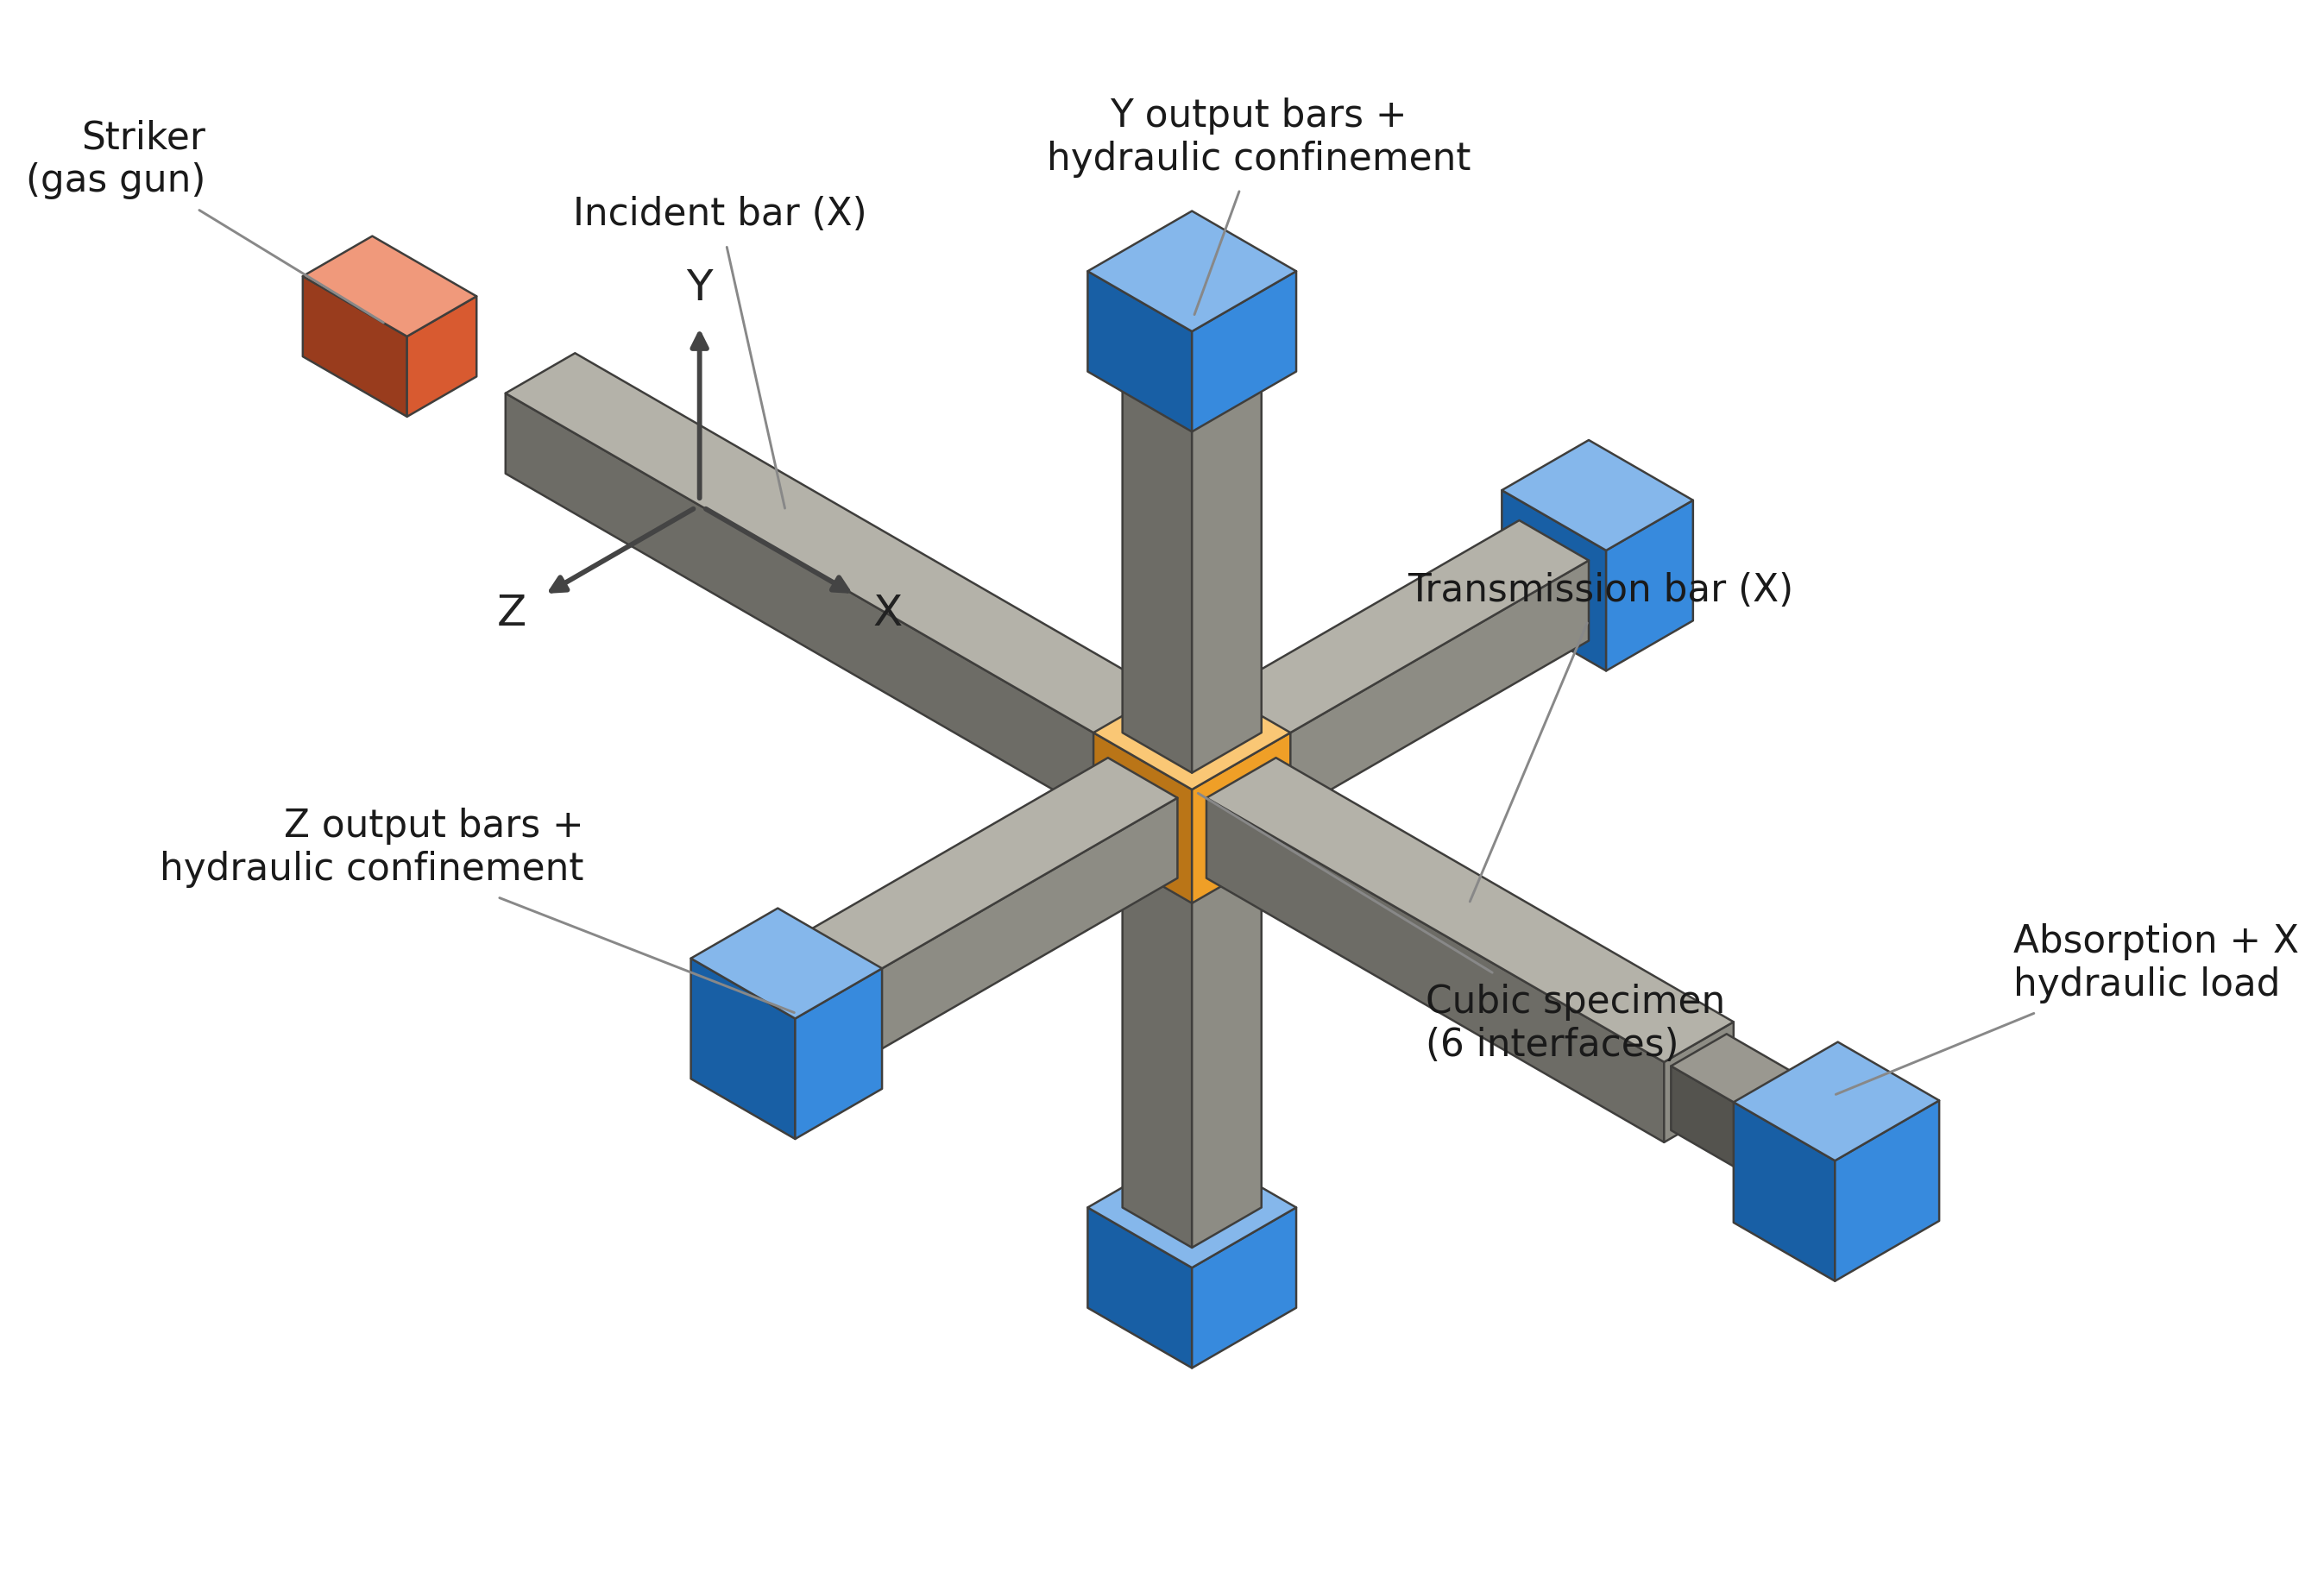
\includegraphics[width=0.92\linewidth]{trihb_system_schematic.png}
  \caption{Isometric schematic of the Monash Tri-HB. The gas gun drives the $X$
  incident/transmission train; two output-bar pairs on $Y$ and $Z$ and a
  hydraulic load cylinder on $X$ apply independent confinement, giving
  static--dynamic coupled true-triaxial loading on the central cubic specimen.}
  \label{fig:schematic}
\end{figure}

\begin{table}[t]
  \centering
  \caption{Representative Monash Tri-HB bar and loading parameters (42CrMo steel).}
  \label{tab:bar}
  \begin{tabular}{lll}
    \toprule
    Quantity & Symbol & Value \\
    \midrule
    Bar density & $\rho_b$ & \SI{7850}{kg/m^3} \\
    Bar Young's modulus & $E_b$ & \SI{210}{GPa} \\
    Bar wave speed & $\Cz$ & \SI{5200}{m/s} \\
    Bar yield strength & $\sigma_y$ & \SI{930}{MPa} \\
    Striker (diameter, length) & $\diameter,\,L_s$ & \SI{40}{mm}, \SI{0.5}{m} \\
    Square-bar cross-section & $A_b$ & \SI{50}{mm}\,$\times$\,\SI{50}{mm} \\
    Incident / transmission / output bar & $L$ & \num{2.5} / \num{2.0} / \SI{2.0}{m} \\
    Maximum impact velocity & $v$ & \SI{50}{m/s} \\
    Hydraulic confinement capacity & $p_c$ & \SI{100}{MPa} \\
    Gauge sampling rate & --- & \SI{1}{MHz} \\
    \bottomrule
  \end{tabular}
\end{table}

\subsection{Loading configurations}

Because each axis carries an independent hydraulic pre-stress, the gas-gun Tri-HB
realises the conventional dynamic-loading cases as special cases of a single
apparatus (Table~\ref{tab:families}): the historical uniaxial SHPB when the
lateral axes are unconfined (Mode~1), axisymmetric confined SHPB when the two
lateral pre-stresses are equal (Mode~2), and genuine true-triaxial
static--dynamic loading when they differ, $\sigma_2\neq\sigma_3$ (Mode~3). Mode~3
is the configuration that distinguishes the system; Modes~1 and~2 are recovered
from it simply by removing or equalising the lateral confinement, which is what
makes uniaxial, confined and true-triaxial results directly comparable on one
apparatus.

The corresponding $p$--$q$ stress paths (Fig.~\ref{fig:modes}) are plotted in
\emph{total} specimen stress, $\sigma=\sigma_{\mathrm{pre}}+\Delta\sigma_{\mathrm{dyn}}$,
not in dynamic increments. The uniaxial case carries no pre-stress and therefore
starts at the origin, whereas the true-triaxial case --- here pre-stressed to
$(\sigma_1,\sigma_2,\sigma_3)=(30,20,15)\,\mathrm{MPa}$, i.e.\ a static point
$(p_0,q_0)\approx(21.7,13.2)\,\mathrm{MPa}$ --- begins at that point and moves
outward as the dynamic $X$ pulse is superposed. The bar-gauge reduction itself
operates on the dynamic increments alone (\S\ref{sec:prestress}); the total state
is plotted because specimen failure is governed by the absolute stress
$\sigma_{\mathrm{pre}}+\Delta\sigma_{\mathrm{dyn}}$, not by the increment, and this
choice is what makes the pre-stress offset of the true-triaxial path physically
meaningful.

\begin{table}[t]
  \centering
  \caption{Loading configurations of the Monash Tri-HB, set by the per-axis
  hydraulic pre-stress.}
  \label{tab:families}
  \small\setlength{\tabcolsep}{6pt}
  \begin{tabular}{cllc}
    \toprule
    Mode & Configuration & Lateral pre-stress & True-triaxial \\
    \midrule
    1 & Uniaxial SHPB & none ($\sigma_2=\sigma_3=0$) & no \\
    2 & Axisymmetric confined SHPB & equal ($\sigma_2=\sigma_3>0$) & partial \\
    3 & Tri-HB static--dynamic & unequal ($\sigma_2\neq\sigma_3$) & yes \\
    \bottomrule
  \end{tabular}
\end{table}

\begin{figure}[t]
  \centering
  \begin{subfigure}[b]{0.49\linewidth}
    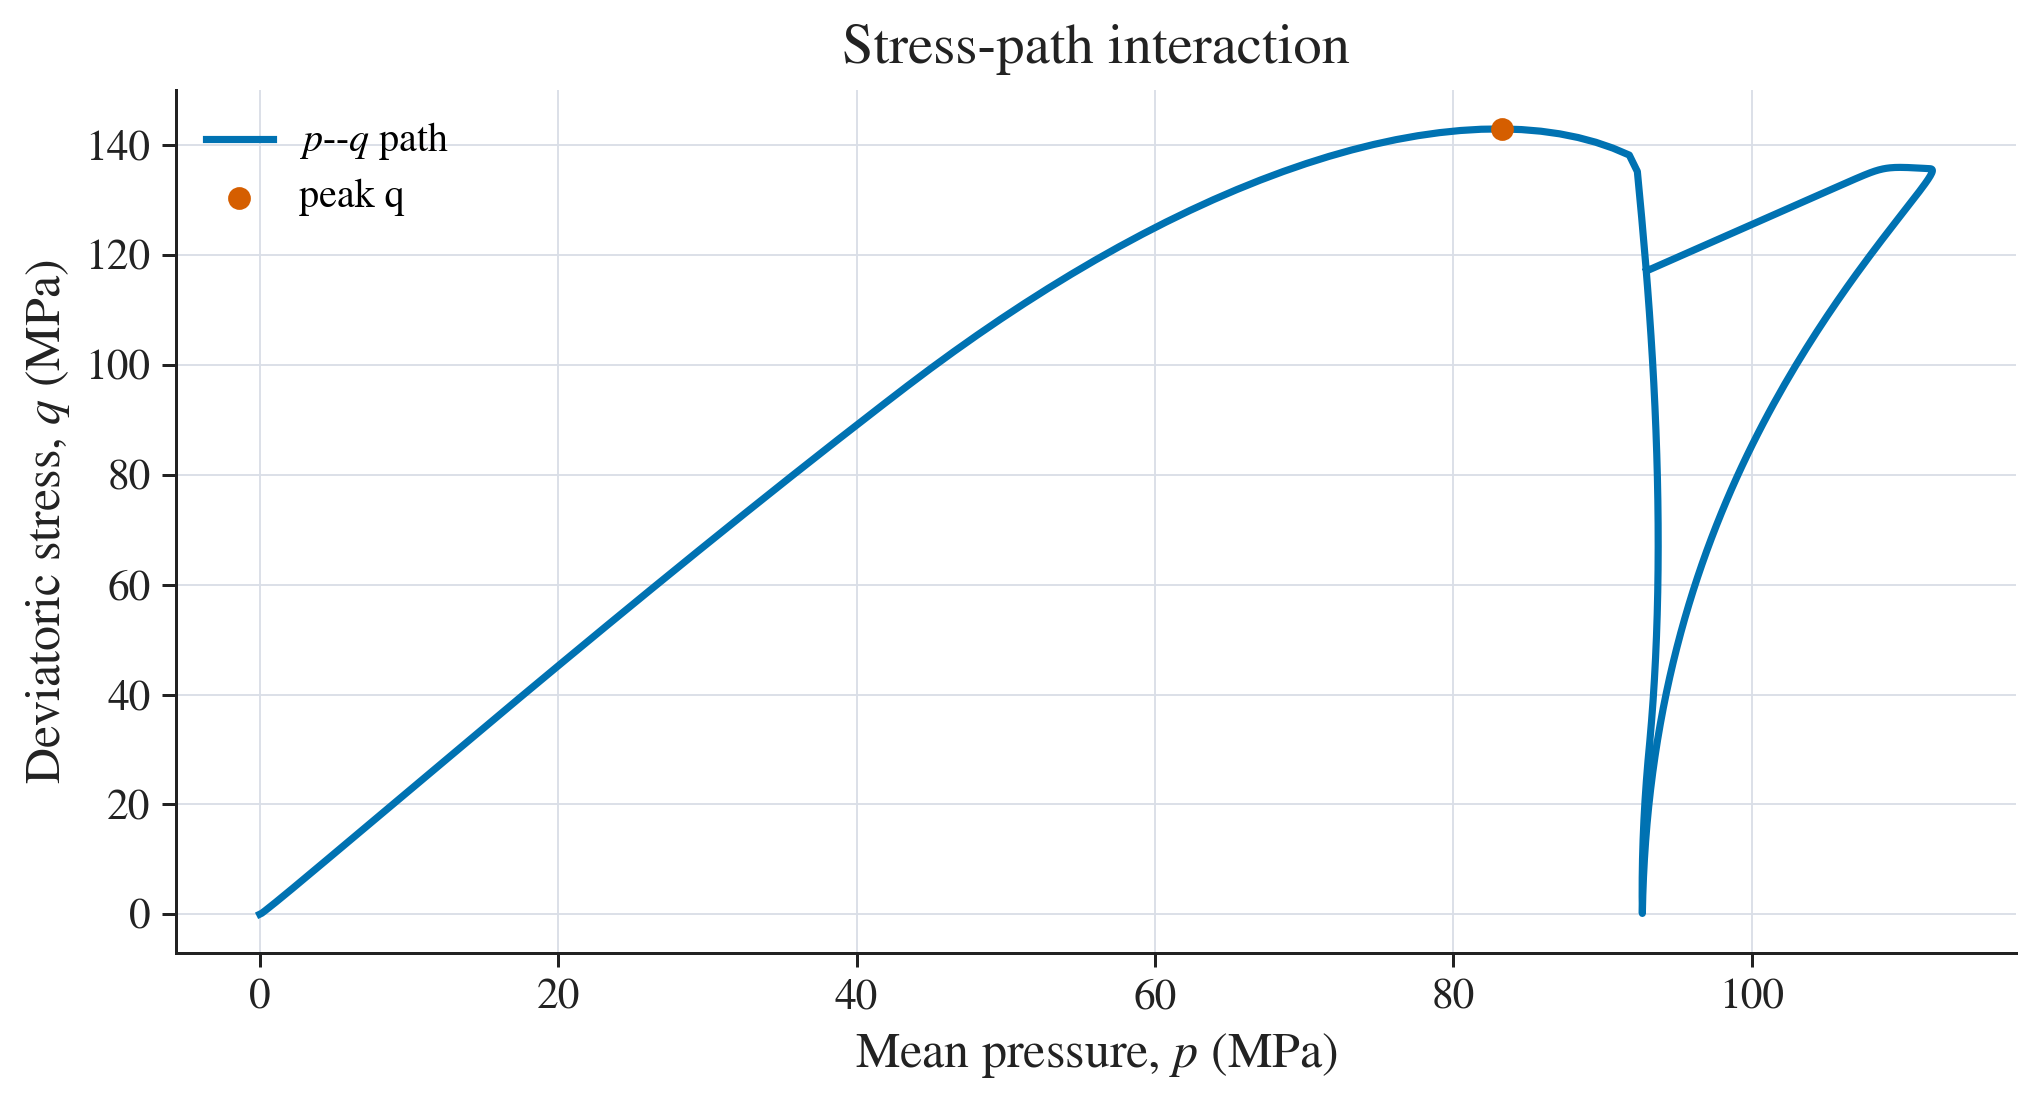
\includegraphics[width=\linewidth]{mode_1_gas_gun_uniaxial_stress_path.png}
    \caption{Mode 1 --- uniaxial SHPB}
  \end{subfigure}\hfill
  \begin{subfigure}[b]{0.49\linewidth}
    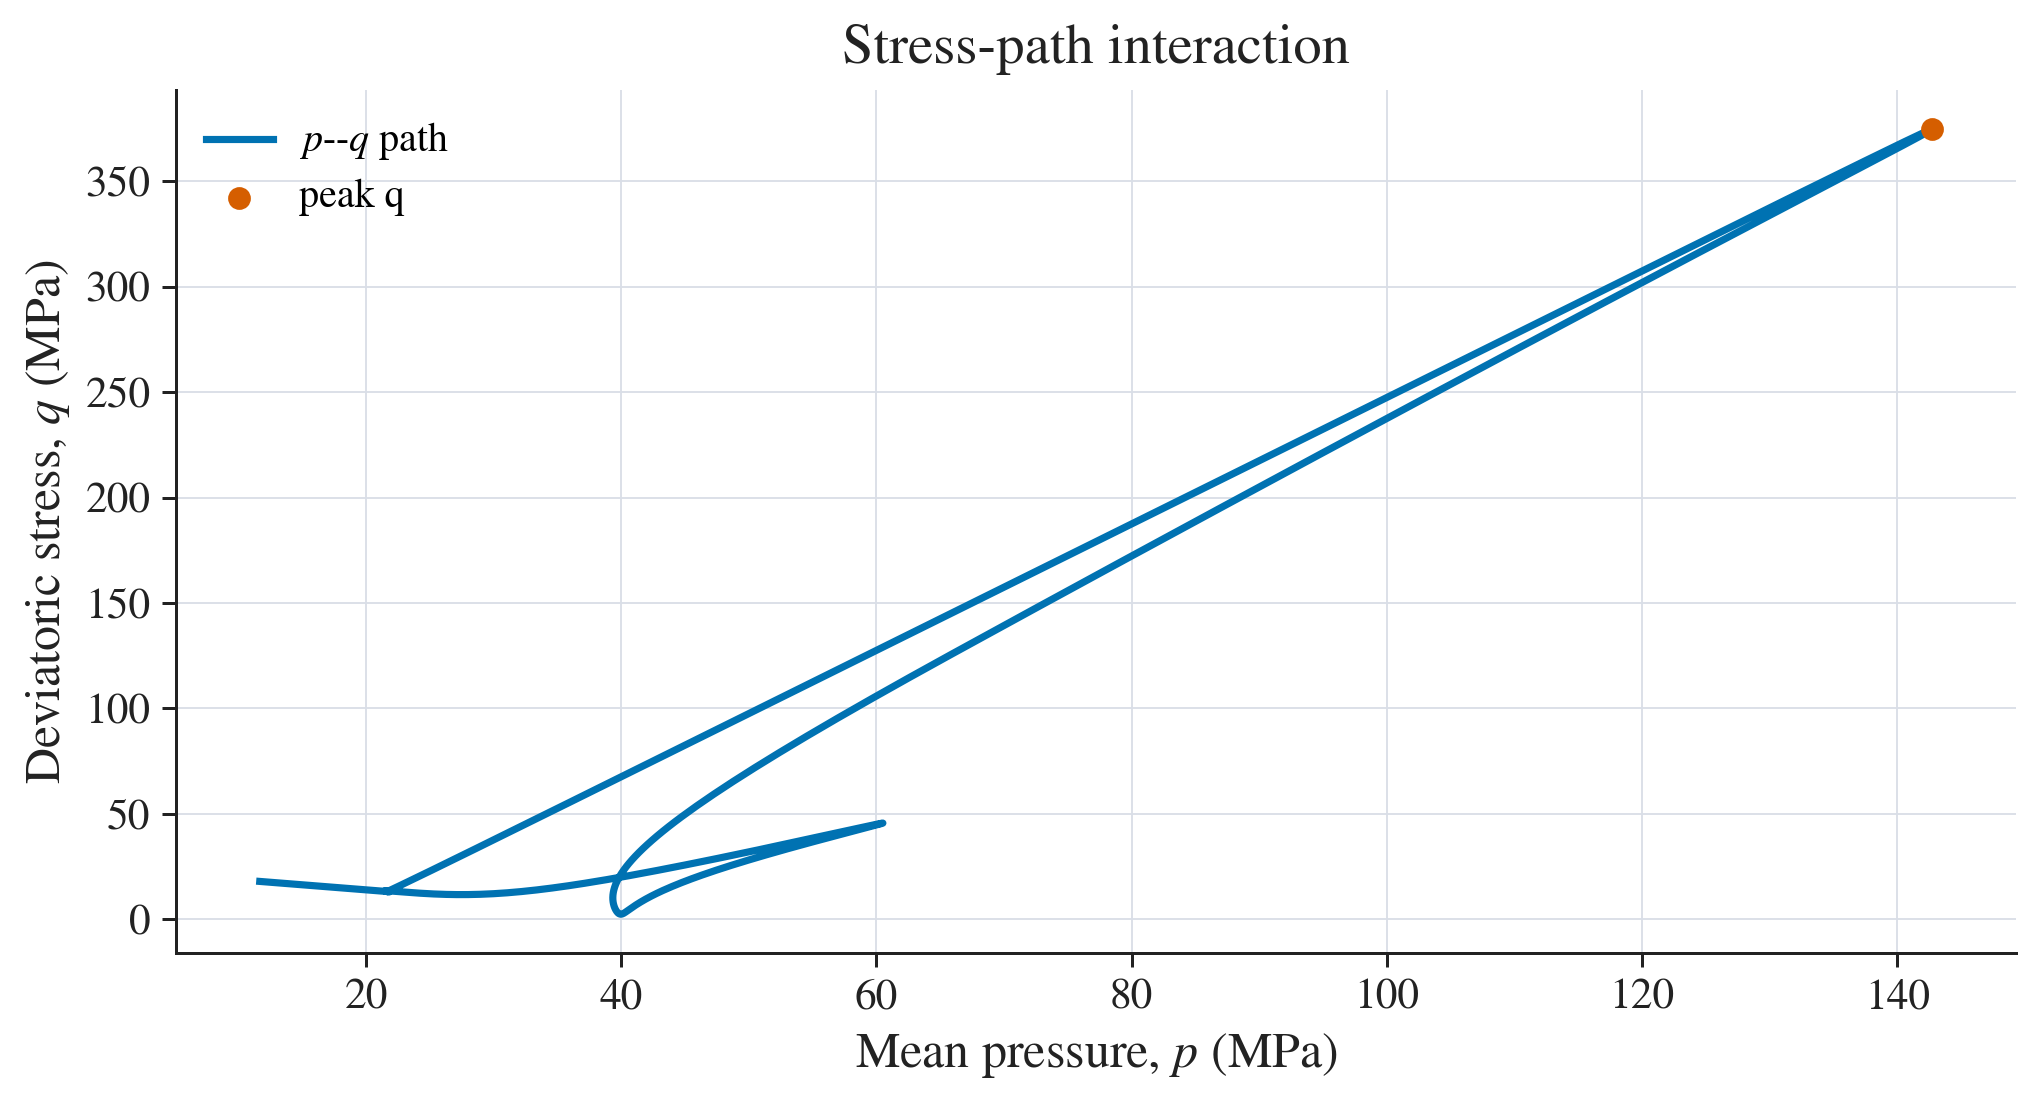
\includegraphics[width=\linewidth]{mode_3_monash_tri_hb_stress_path.png}
    \caption{Mode 3 --- true-triaxial Tri-HB}
  \end{subfigure}
  \caption{Mean-pressure--deviatoric-stress ($p$--$q$) trajectories for the
  uniaxial (a) and true-triaxial (b) configurations of the Tri-HB, plotted in
  \emph{total} specimen stress
  $\sigma=\sigma_{\mathrm{pre}}+\Delta\sigma_{\mathrm{dyn}}$ (see text). Uniaxial
  loading (a) carries no pre-stress and traces a steep deviatoric path from the
  origin; the true-triaxial case (b), pre-stressed to $(30,20,15)$~MPa, begins at
  its static point and populates the multiaxial $p$--$q$ plane. The spread of
  accessible stress paths, set by the per-axis pre-stress, is the analytical
  advantage of the system.}
  \label{fig:modes}
\end{figure}

\section{Wave propagation and per-axis data reduction}\label{sec:reduction}

\paragraph{Sign and notation conventions.} We adopt the compression-positive
convention standard in rock dynamics: normal stress and strain are positive in
compression, and the particle velocity $v$ is positive along $+x$, the
incident-pulse propagation direction. The recorded bar-gauge strains are
accordingly $\eps_{\mathrm{in}}>0$ (compressive incident), $\eps_{\mathrm{re}}<0$
(tensile reflected, for a specimen softer than the bars) and
$\eps_{\mathrm{tr}}>0$ (compressive transmitted). Principal stresses are ordered
$\sigma_1\ge\sigma_2\ge\sigma_3$ and $\langle x\rangle=\max(x,0)$ denotes the
Macaulay bracket.

\subsection{One-dimensional wave propagation and dispersion}\label{sec:wave}

Each pressure bar is a long, slender rod in which, for wavelengths much greater
than the bar diameter, the axial displacement $u(x,t)$ obeys the
one-dimensional elastic wave equation
\begin{equation}
\frac{\partial^2 u}{\partial t^2}=\Cz^2\,\frac{\partial^2 u}{\partial x^2},
\qquad \Cz=\sqrt{E_b/\rho_b},
\label{eq:wave}
\end{equation}
whose general d'Alembert solution $u=f(x-\Cz t)+g(x+\Cz t)$ superposes
forward- and backward-travelling parts. For a single travelling wave the axial
strain and particle velocity are proportional, giving the Hopkinson identity
\begin{equation}
v(x,t)=\pm\,\Cz\,\eps(x,t),
\label{eq:hopkinson}
\end{equation}
with the upper (lower) sign for a wave travelling in the $+x$ ($-x$) direction
under the compression-positive convention above; a resistance gauge that measures
strain therefore also measures the particle velocity through the bar wave speed.
Summing the incident ($+x$) and reflected ($-x$) contributions then yields the
face velocities of Eq.~\eqref{eq:faces}.

At a planar interface between media of acoustic impedance $Z=\rho c$, continuity
of traction and velocity gives the stress reflection and transmission
coefficients\footnote{For a 42CrMo steel bar
$Z_b=\rho_b\Cz\approx4.06\times10^{7}\,\mathrm{kg\,m^{-2}\,s^{-1}}$.}
\begin{equation}
R=\frac{\sigma_R}{\sigma_I}=\frac{Z_2-Z_1}{Z_1+Z_2},\qquad
T=\frac{\sigma_T}{\sigma_I}=\frac{2Z_2}{Z_1+Z_2}.
\label{eq:fresnel}
\end{equation}
For a rock specimen softer than the steel bars ($Z_s<Z_b$) the reflection
coefficient is negative, so the reflected pulse is tensile --- the origin of the
negative reflected strain $\eps_{\mathrm{re}}$ recorded in compression tests, and
a sign-diagnostic of the impedance match.

Equation~\eqref{eq:wave} is exact only in the long-wavelength limit. The exact
axisymmetric (Pochhammer--Chree) solution makes the phase velocity
frequency-dependent, $c_\phi(ka)=\Cz\,\Phi(ka,\nu_b)$, where $k$ is the wavenumber
and $a$ the bar radius: $\Phi\approx1$ for $ka\lesssim0.1$ but falls by a few
percent as $ka\to1$, so an unshaped rectangular pulse --- rich in high-$ka$
harmonics --- develops spurious oscillations as it travels. Dispersion is
negligible while the rise time $\tau_r$ satisfies $a/(c_\phi\tau_r)\lesssim0.1$.
The Tri-HB therefore uses a pulse-shaped, half-sine incident wave, which
concentrates its energy at $ka\ll1$ and is essentially dispersion-free for the
bar geometries used here; the computational workspace represents the loading with
a smooth half-sine incident wave for the same reason.

\subsection{Force--velocity continuity and the three-wave method}

At the incident-bar/specimen face the bar carries the superposed incident and
reflected waves, while the transmission bar carries only the outgoing wave, so the
two face forces and velocities are
\begin{equation}
F_1=E_bA_b\,(\eps_{\mathrm{in}}+\eps_{\mathrm{re}}),\quad
v_1=\Cz(\eps_{\mathrm{in}}-\eps_{\mathrm{re}});\qquad
F_2=E_bA_b\,\eps_{\mathrm{tr}},\quad
v_2=\Cz\,\eps_{\mathrm{tr}}.
\label{eq:faces}
\end{equation}
The average axial stress, strain rate and strain follow from \eqref{eq:faces}. In
general --- valid at \emph{all} times, equilibrium or not --- the two-wave forms are
\begin{align}
\sigma_x(t) &= \frac{F_1+F_2}{2A_s}=\frac{E_b A_b}{2 A_s}\big(\eps_{\mathrm{in}}+\eps_{\mathrm{re}}+\eps_{\mathrm{tr}}\big), \label{eq:twowave}\\
\epsd(t)    &= \frac{v_1-v_2}{L_s}=\frac{\Cz}{L_s}\big(\eps_{\mathrm{in}}-\eps_{\mathrm{re}}-\eps_{\mathrm{tr}}\big), \qquad
\eps(t)=\int_0^t \epsd\,\mathrm{d}\tau, \label{eq:srate}
\end{align}
where $A_b,A_s$ are the bar and specimen cross-sections and $L_s$ the specimen
length. Only once the specimen has reverberated into dynamic stress equilibrium
($t\gtrsim 3\,t_{\mathrm{travel}}$, $t_{\mathrm{travel}}=L_s/c_p$) do the two face
forces equalise, $\eps_{\mathrm{in}}+\eps_{\mathrm{re}}=\eps_{\mathrm{tr}}$, and
only then do \eqref{eq:twowave}--\eqref{eq:srate} reduce to the familiar one-wave
relations
\begin{equation}
\sigma_x(t)=\frac{E_b A_b}{A_s}\,\eps_{\mathrm{tr}}(t),\qquad
\epsd(t)=-\frac{2\Cz}{L_s}\,\eps_{\mathrm{re}}(t).
\label{eq:onewave}
\end{equation}
Agreement between the two-wave and one-wave forms is the reducer's built-in
equilibrium check; equilibrium itself is quantified by the force-balance ratio
\begin{equation}
\mathcal{R}(t)=\frac{|F_1(t)-F_2(t)|}{\tfrac12\big(|F_1(t)|+|F_2(t)|\big)}<0.05,
\qquad t_{\mathrm{eq}}\approx(3\text{--}5)\,L_s/c_p,
\label{eq:equil}
\end{equation}
the force magnitudes in the denominator keeping $\mathcal{R}$ well-defined through
the early transient.
The lateral response is obtained from the two output bars on each transverse
axis. Each transverse axis is instrumented symmetrically with two output
(transmission) bars that carry only outgoing waves, so each output-bar face force
and velocity are $E_bA_b\,\eps_{yk}$ and $\Cz\,\eps_{yk}$ ($k=1,2$). Under the
standard one-dimensional wave assumption with symmetric lateral loading --- planar
(rigid) specimen faces, no interface rotation and negligible transverse inertia
--- averaging the two opposing faces gives the lateral stress, while the rate at
which the specimen widens against its lateral dimensions $d_y,d_z$ gives the
lateral strain rate,
\begin{align}
\sigma_y &=\frac{E_b A_b}{2A_s}\big(\eps_{y1}+\eps_{y2}\big), &
\sigma_z &=\frac{E_b A_b}{2A_s}\big(\eps_{z1}+\eps_{z2}\big), \\
\epsd_y  &=-\frac{\Cz}{d_y}\big(\eps_{y1}+\eps_{y2}\big), &
\epsd_z  &=-\frac{\Cz}{d_z}\big(\eps_{z1}+\eps_{z2}\big),
\label{eq:lateral}
\end{align}
with $A_s$ here the loaded lateral area and $\eps_{y}=\int_0^t\epsd_y\,\mathrm{d}\tau$.
The minus sign reflects the convention: under axial compression both output bars
recede as the specimen expands laterally, an outward (compression-negative,
i.e.\ extensile) lateral strain. These lateral outputs are Poisson-driven --- the
$X$ pulse compresses the specimen, which expands laterally and drives output
waves outward along the $Y$ and $Z$ bars, recorded by gauges G3--G6 --- and the
Virtual Tri-HB performs the reduction simultaneously on all three axes, so a
single test yields the full $\sigma_x,\sigma_y,\sigma_z$ history rather than one
axial curve.

\subsection{Validity of the three-wave method under static pre-stress}\label{sec:prestress}

In the static--dynamic configuration the hydraulic cylinders pre-load the bars
before the pulse arrives, so the bar ends are no longer free. Because the bar is
linear-elastic, the total field superposes a uniform static part and the
propagating dynamic part, $\sigma=\sigma_s+\sigma_d$ with
$\sigma_s=F_{\mathrm{pre}}/A_b=\mathrm{const}$ ($\mathrm{d}\sigma_s/\mathrm{d}x=0$).
Substituting into \eqref{eq:wave}, the static part drops out and the dynamic part
obeys the same wave equation, so the three-wave relations apply unchanged to the
dynamic \emph{increments} $\eps_{\mathrm{in}},\eps_{\mathrm{re}},\eps_{\mathrm{tr}}$
--- the pre-stress is merely a constant gauge offset, removed by baselining before
the pulse. The superposition is valid provided the bar stays elastic at all times,
\begin{equation}
\sigma_{d,\mathrm{peak}}<\sigma_{\mathrm{prop}}-|\sigma_s|,
\label{eq:budget}
\end{equation}
so the pre-stress consumes part of the dynamic-amplitude budget (the bar-plasticity
limit the workspace enforces). The bar--specimen interfaces, being unilateral, must
also stay in contact: a reflected tensile excursion must not exceed the static
pre-compression, $|\sigma_d|\le\sigma_s$, or the contact separates and the boundary
condition turns nonlinear --- here the pre-stress \emph{helps}, holding the
interfaces closed. The far ends now carry a static force, but the reflection a pulse
sees there is governed by the termination's \emph{dynamic} impedance, not by that
force, and is in any case delayed beyond the measurement window by the bar length.

The constancy of the \emph{bar} properties is what makes this robust. The bar wave
speed is pre-stress-independent to within a sub-percent acoustoelastic shift,
$\Delta C_0/C_0\approx(\beta/E_b)\,\sigma_s\lesssim0.3\%$ with
$\beta=\mathcal{O}(1$--$5)$ for steel, so $E_b,C_0,A_b$ may be treated as constants
and the bar-based reduction holds at every confinement. The \emph{specimen}, by
contrast, is genuinely pre-stress-dependent: confinement closes microcracks and
stiffens the rock, so $E_s=E_s(p)$ and $c_p=c_p(p)$ can vary by tens of percent
over the first tens of megapascals. This is precisely the response the test
measures, but it means any specimen-property-based output --- the equilibrium window
$t_{\mathrm{eq}}\propto L_s/c_p$ and the energy partition --- must
use the \emph{confined} values; and under true-triaxial pre-stress the closure is
directional, rendering the rock elastically anisotropic
($c_{p,x}\neq c_{p,y}\neq c_{p,z}$), a stress-induced anisotropy the three
orthogonal bars can resolve. This clean separation --- a linear,
pre-stress-independent bar reduction carrying a nonlinear, pre-stress-dependent
specimen response --- is what legitimises and gives meaning to static--dynamic
coupled testing.

Finally, the sandwiched specimen itself does \emph{not} superpose --- it is the
nonlinear element. The bars still record the true dynamic increments, but those
increments are the rock's response at its \emph{pre-stressed} tangent, which is the
coupling the test measures; the specimen's absolute state is the static pre-load
plus that increment,
$\sigma_{\mathrm{total}}=\sigma_{\mathrm{pre}}+\Delta\sigma_{\mathrm{dyn}}$ and
$\varepsilon_{\mathrm{total}}=\sigma_{\mathrm{pre}}/E_s(p)+\Delta\varepsilon_{\mathrm{dyn}}$,
so only the strain reconstruction draws on the confined modulus $E_s(p)$ (the
bar-based stress increment is self-contained). Confinement moreover \emph{eases}
the measurement: as crack closure raises $c_{p,s}$ and hence $Z_s=\rho_s c_{p,s}$,
the equilibration time $t_{\mathrm{eq}}\propto L_s/c_{p,s}$ shortens and the
bar--specimen impedance mismatch $|R|=(Z_b-Z_s)/(Z_b+Z_s)$ falls, giving a cleaner
transmitted signal (at the cost of a weaker reflected one).

\section{The integrated computational workspace}\label{sec:twin}

The Virtual Tri-HB (\texttt{tri\_hb\_integrated.py}) is a single application that
bundles six analysis steps under one shared experimental setup: (1) configuration
and either simulation or reduction of bar-gauge data; (2) wave-propagation and
equilibrium analysis; (3) stress-path and invariant analysis; (4) damage and
energy analysis with directional descriptors; (5) a publication-ready summary;
and (6) automatic generation of a report and presentation (\LaTeX{} + PDF) from
the current run. A separate page renders the live calibration/validation plan.
Each step inherits the shared configuration, so the wave, stress-path and damage
views remain mutually consistent. The stress-path stage resolves the total
stresses into the invariants
\begin{equation}
p=\tfrac{1}{3}(\sigma_x+\sigma_y+\sigma_z),\qquad
q=\sqrt{3J_2},\qquad
\cos 3\theta=\frac{3\sqrt3}{2}\frac{J_3}{J_2^{3/2}},
\label{eq:invariants}
\end{equation}
where $s_{ij}=\sigma_{ij}-p\,\delta_{ij}$ is the deviatoric stress,
$J_2=\tfrac12 s_{ij}s_{ij}=\tfrac16\big[(\sigma_x-\sigma_y)^2+(\sigma_y-\sigma_z)^2+(\sigma_z-\sigma_x)^2\big]$
and $J_3=\det(s_{ij})=s_1s_2s_3$ are its second and third invariants. With compression positive and the ordering
$\sigma_1\ge\sigma_2\ge\sigma_3$, the Lode angle $\theta\in[0^\circ,60^\circ]$
runs from the triaxial-compression meridian ($\theta=0^\circ$, $\sigma_2=\sigma_3$)
to the triaxial-extension meridian ($\theta=60^\circ$, $\sigma_1=\sigma_2$), so
that all three principal stresses --- including the intermediate stress
$\sigma_2$ through $\theta$ --- enter the subsequent failure analysis
(Fig.~\ref{fig:stresspath}).

\begin{figure}[t]
  \centering
  \begin{subfigure}[b]{0.49\linewidth}
    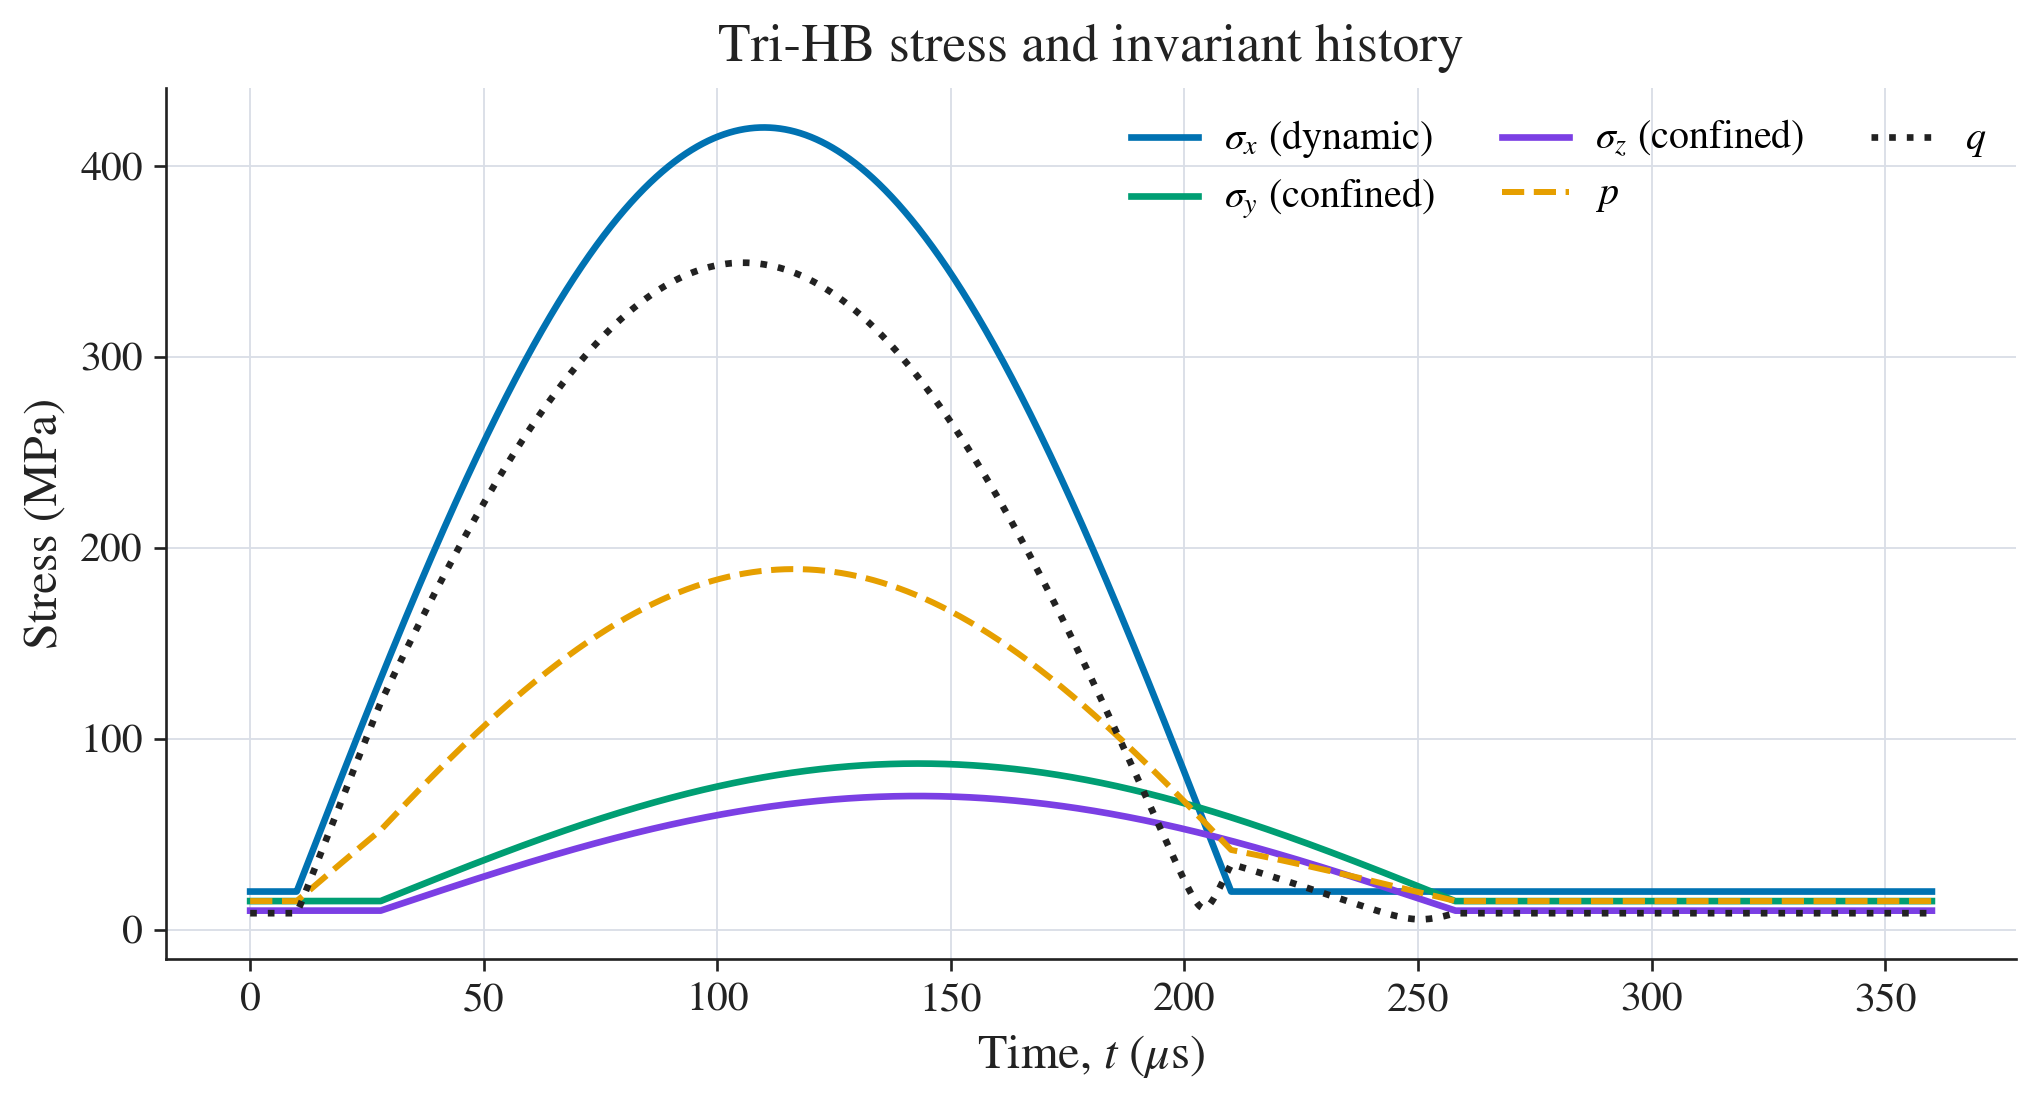
\includegraphics[width=\linewidth]{trihb_stress_invariants.png}
    \caption{Stress and invariant histories}
  \end{subfigure}\hfill
  \begin{subfigure}[b]{0.49\linewidth}
    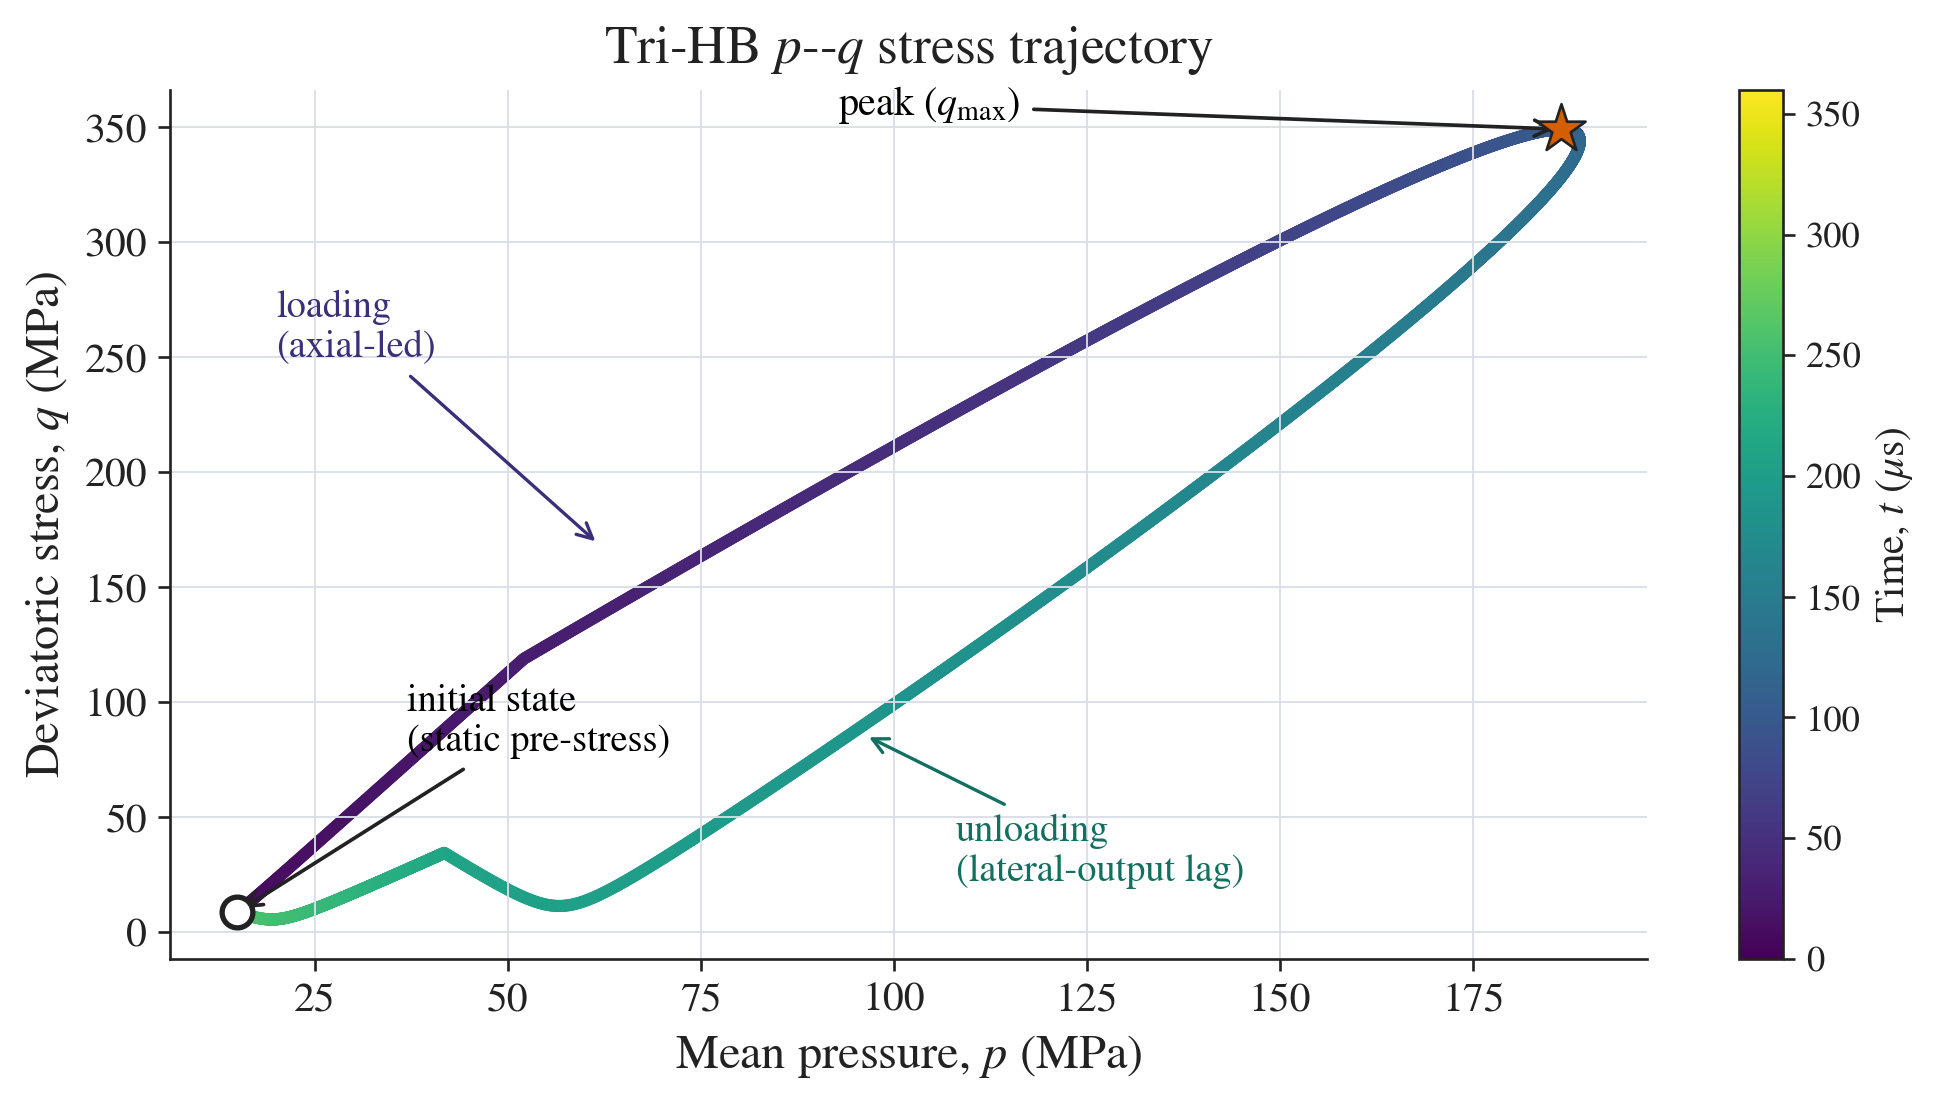
\includegraphics[width=\linewidth]{trihb_pq_trajectory.png}
    \caption{$p$--$q$ trajectory (time-coloured)}
  \end{subfigure}
  \caption{Stress-path analysis (Step~3) for the gas-gun Tri-HB (Mode~3): a
  dynamic $X$ pulse superposed on a true-triaxial static pre-stress, with the
  Poisson-driven lateral output recorded on the $Y$ and $Z$ bars. (a) Total
  principal stresses with the mean ($p$) and deviatoric ($q$) invariants; (b) the
  resulting $p$--$q$ trajectory (total stress, time-coloured), annotated with the
  initial static-pre-stress state, the axial-led loading branch, the deviatoric
  peak, and the lower unloading branch produced by the axial--lateral timing lag.}
  \label{fig:stresspath}
\end{figure}

The time-coloured $p$--$q$ trajectory (Fig.~\ref{fig:stresspath}b) makes the
loading history explicit and, like Fig.~\ref{fig:modes}, is drawn in \emph{total}
stress $\sigma=\sigma_{\mathrm{pre}}+\Delta\sigma_{\mathrm{dyn}}$. Four stages are
visible. (i)~The path \emph{begins at the static pre-stress point} $(p_0,q_0)$ set
by the true-triaxial confinement, not at the origin. (ii)~As the dynamic $X$ pulse
arrives, the axial stress rises ahead of the Poisson-driven lateral outputs ---
which reach the $Y,Z$ output bars only after a finite lateral transit --- so the
early path is \emph{axial-led}: $q$ climbs steeply along the upper (loading)
branch with comparatively little change in $p$. (iii)~At the pulse crest the
trajectory reaches \emph{peak} deviatoric stress $q_{\max}$, where the failure
index $F=q/q_f$ is largest. (iv)~As the pulse \emph{unloads}, the axial stress
relaxes before the lagged lateral outputs decay, so the return follows a distinct
\emph{lower} (unloading) branch and the trajectory does not retrace itself before
settling back to the static point. The open loop between the two branches is
therefore a \emph{timing} effect --- the phase lag between the prescribed axial
pulse and the Poisson lateral outputs --- and not a plastic or damage hysteresis:
because the stresses are prescribed they return to the pre-stress state, while the
irreversible response appears instead in the strain, stiffness and damage
histories (\S\ref{sec:energy}--\ref{sec:ortho}). With independent stress and
strain measured on each axis, the experiment will resolve whether the true
material response adds genuine (dissipative) hysteresis to this kinematic loop.

\section{Constitutive advances}\label{sec:advances}

\subsection{True-triaxial, rate-dependent failure envelope}\label{sec:env}

Failure is evaluated through the index $F=q/q_f$ against a pressure-dependent
envelope with a deviatoric (Lode) shape and an optional rate dependence,
\begin{equation}
q_f=(A_{\mathrm{eff}}+B_{\mathrm{eff}}\,p^{\,n})\,h(\theta),\qquad
A_{\mathrm{eff}}=A\cdot\mathrm{DIF}_c,
\label{eq:qf}
\end{equation}
with the (compression) dynamic increase factor $\mathrm{DIF}_c$ defined in
Eq.~\eqref{eq:difc} below.
The meridian parameters are not free. Requiring the envelope to reproduce the
Step-1 strength law $\sigma_1=(\mathrm{UCS}+k_{\mathrm{conf}}\sigma_3)\,\mathrm{DIF}_c$
in triaxial compression ($\theta=0$, $h=1$, $n=1$) and eliminating $\sigma_3$
through $p$ and $q$ yields the linear Mohr--Coulomb meridian
\begin{equation}
A=\frac{3\,\mathrm{UCS}}{k_{\mathrm{conf}}+2},\qquad
B=\frac{3\,(k_{\mathrm{conf}}-1)}{k_{\mathrm{conf}}+2},\qquad n=1,
\label{eq:AB}
\end{equation}
so that $F=q/q_f=1$ at the static failure point by construction (verified to
machine precision for all confinement ratios $k_{\mathrm{conf}}$). The exponent
$n$ is a fitting parameter for curved meridians; $B_{\mathrm{eff}}$ then carries
units of $\mathrm{MPa}^{1-n}$ so that $q_f$ remains a stress for any $n$, with
$n=1$ the default linear case. The deviatoric shape $h(\theta)$ admits three forms: a legacy cap, a
linear extension-weakened interpolation, and a convex Willam--Warnke
form~\citep{willam1975}. Both new forms use the meridian ratio $\rho_t/\rho_c$
and make the extension meridian \emph{weaker} than compression --- the physically
correct sense for brittle rock --- so the intermediate principal stress effect
enters with the right sign (Fig.~\ref{fig:envelope}a). The default is the Lode
form with $\rho_t/\rho_c=0.70$. The optional rate factor $\mathrm{DIF}_c$ inflates
the envelope with strain rate (Fig.~\ref{fig:envelope}b) so that the failure
\emph{onset} shifts dynamically, complementing the rate sensitivity of the damage
kinetics. Rather than a single semi-logarithmic slope~\citep{zhao2000}, we adopt
the experimentally fitted, piecewise dynamic increase factor
of~\citet{ZHU2024105948} --- a static log-linear branch below a transition strain
rate and a power-law dynamic branch above it,
\begin{equation}
\mathrm{DIF}_c=
\begin{cases}
k_c\log_{10}\dot\varepsilon+b, & \dot\varepsilon<10~\mathrm{s^{-1}},\\[3pt]
k_c\log_{10}\dot\varepsilon+b-\dfrac{10^{\beta}}{\alpha}+\dfrac{\dot\varepsilon^{\,\beta}}{\alpha}, & \dot\varepsilon\ge10~\mathrm{s^{-1}},
\end{cases}
\label{eq:difc}
\end{equation}
\begin{equation}
\mathrm{DIF}_t=
\begin{cases}
k_t\log_{10}\dot\varepsilon+b, & \dot\varepsilon<1~\mathrm{s^{-1}},\\[3pt]
k_t\log_{10}\dot\varepsilon+b-\dfrac{1}{\alpha}+\dfrac{\dot\varepsilon^{\,2\beta}}{\alpha}, & \dot\varepsilon\ge1~\mathrm{s^{-1}},
\end{cases}
\label{eq:dift}
\end{equation}
where $\mathrm{DIF}_c,\mathrm{DIF}_t$ are the compression and tension factors,
$\dot\varepsilon$ is the strain rate (s$^{-1}$), $k_c,k_t$ the static gradient
coefficients, $b$ a fitting constant, and $\alpha=10$, $\beta=0.57$; the
inflection (transition) rates are $10~\mathrm{s^{-1}}$ in compression and
$1~\mathrm{s^{-1}}$ in tension. Because the rate effect below the transition is
small, the static branch is taken rate-independent ($k_c=k_t=0$, $b=1$), so
$\mathrm{DIF}=1$ below the transition and rises as a power law above it
(Fig.~\ref{fig:envelope}b); $\mathrm{DIF}_c$ scales the compressive envelope and
$\mathrm{DIF}_t$ the tensile strength used in the directional damage of
\S\ref{sec:ortho}.

The Mohr--Coulomb meridian is adopted as the \emph{default} not because rock is
assumed insensitive to the intermediate principal stress, but because the surface
is written in the standard invariant decomposition
$q_f(p,\theta)=[\,\text{meridian}(p)\,]\,h(\theta)$, in which $\sigma_2$ enters
through the Lode angle $\theta$ (Eq.~\eqref{eq:invariants}) --- that is, through the
deviatoric shape $h(\theta)$, not through the meridian. The meridian only fixes the
compression reference ($\theta=0$, $\sigma_2=\sigma_3$), while the
$\sigma_2$-dependence is carried by $h(\theta)$, exactly as in the
Willam--Warnke~\citep{willam1975} and related meridian--deviatoric criteria. The
linear Mohr--Coulomb meridian is chosen for that reference because it is the
minimal, identifiable form that reduces \emph{exactly} to the routinely measured
unconfined strength and confinement (Mode~2) series, makes the surface consistent
with the Step-1 stress--strain model ($F=1$ at peak), and needs no true-triaxial
data to instantiate --- a calibration anchor available \emph{before} the full
true-triaxial campaign, not a claim that $\sigma_2$ is unimportant.

For studies that target the intermediate-stress effect directly, this default can
be \emph{replaced} by a criterion that depends on $\sigma_2$ intrinsically. The
workspace offers two such calibrated true-triaxial criteria --- Mogi--Coulomb and
modified Lade --- which \S\ref{sec:criteria} details, compares with the default,
and applies to the Tri-HB stress path; ultimately the meridian, the Lode ratio
$\rho_t/\rho_c$ and the criterion choice are all to be \emph{fitted} to the
Tri-HB's own true-triaxial data, the measurement the system is built to provide.

\begin{figure}[t]
  \centering
  \begin{subfigure}[b]{0.49\linewidth}
    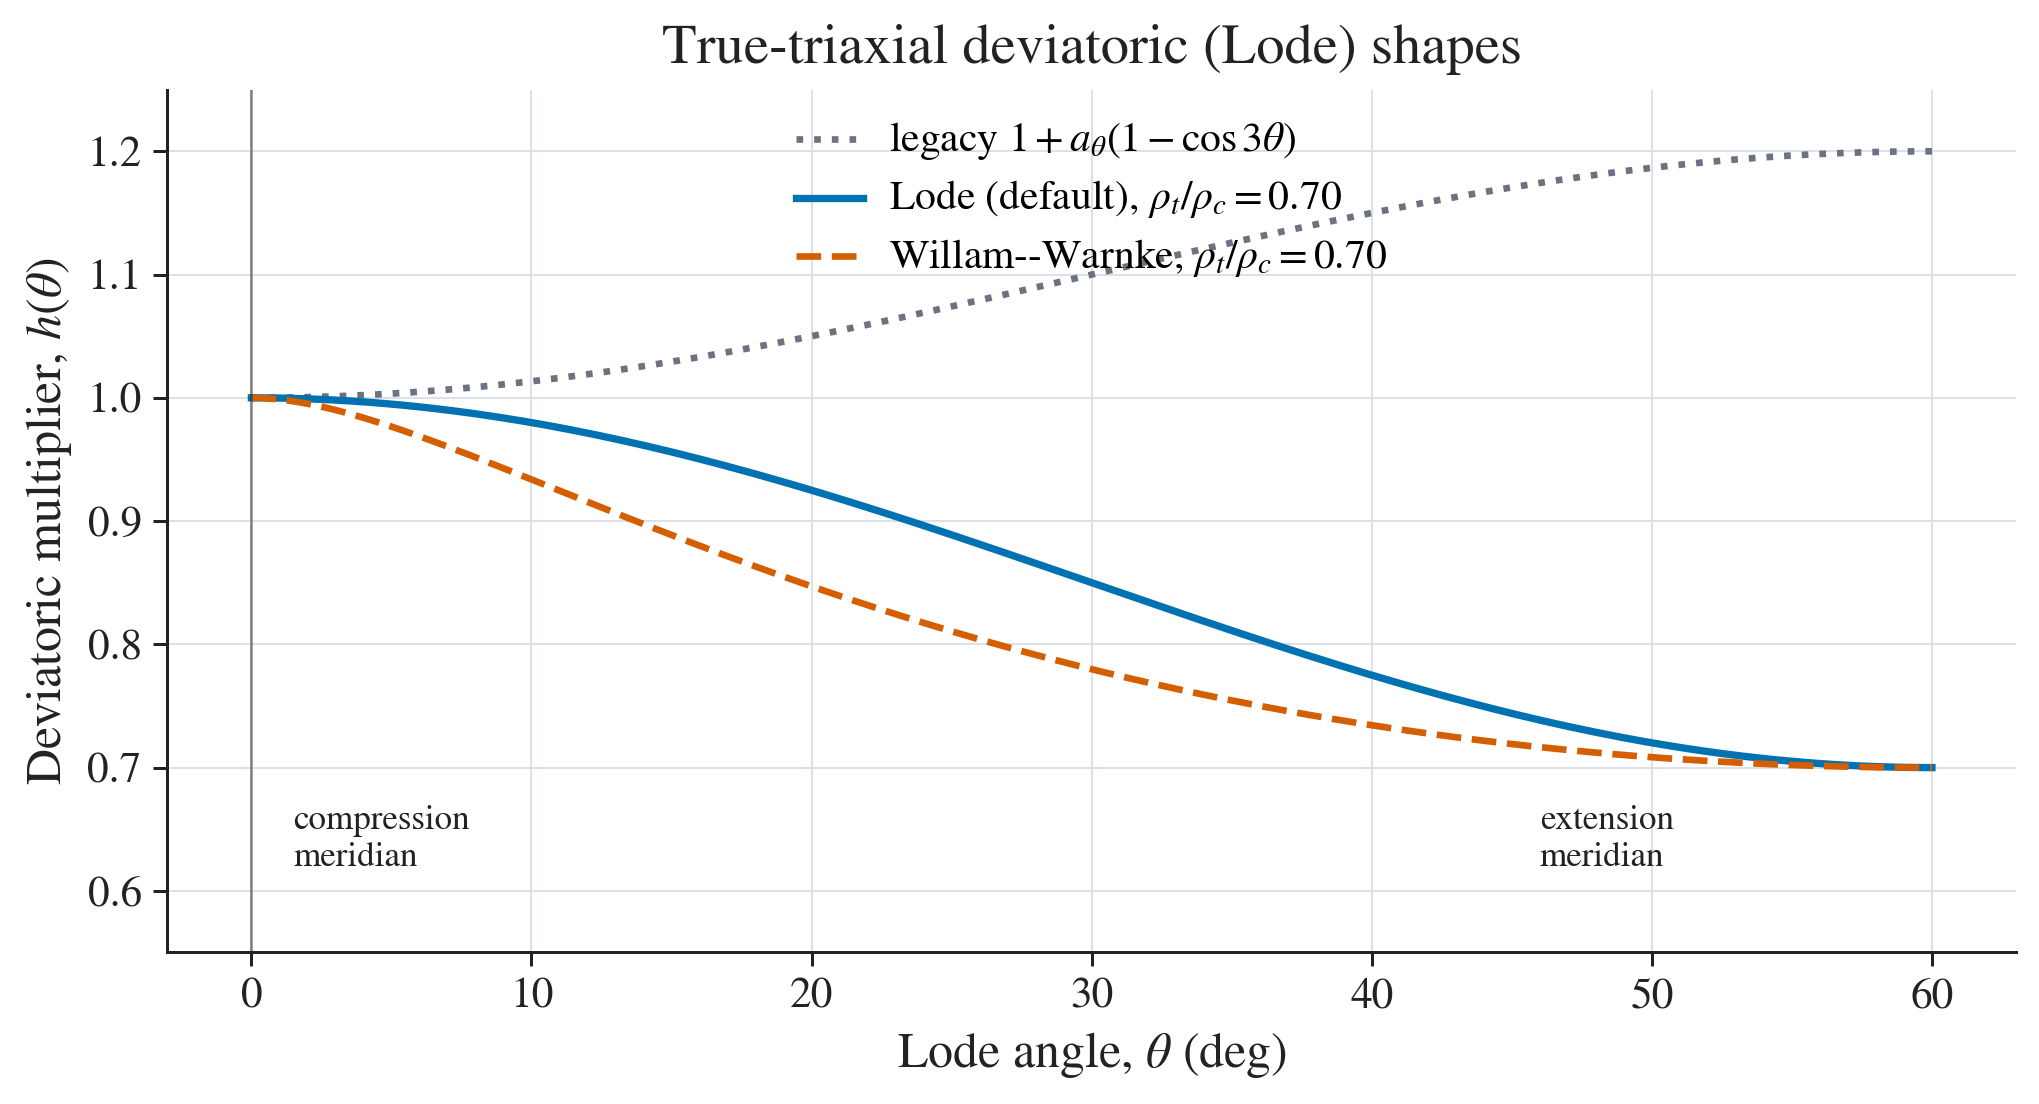
\includegraphics[width=\linewidth]{step3_lode_shapes.png}
    \caption{Deviatoric (Lode) shapes}
  \end{subfigure}\hfill
  \begin{subfigure}[b]{0.49\linewidth}
    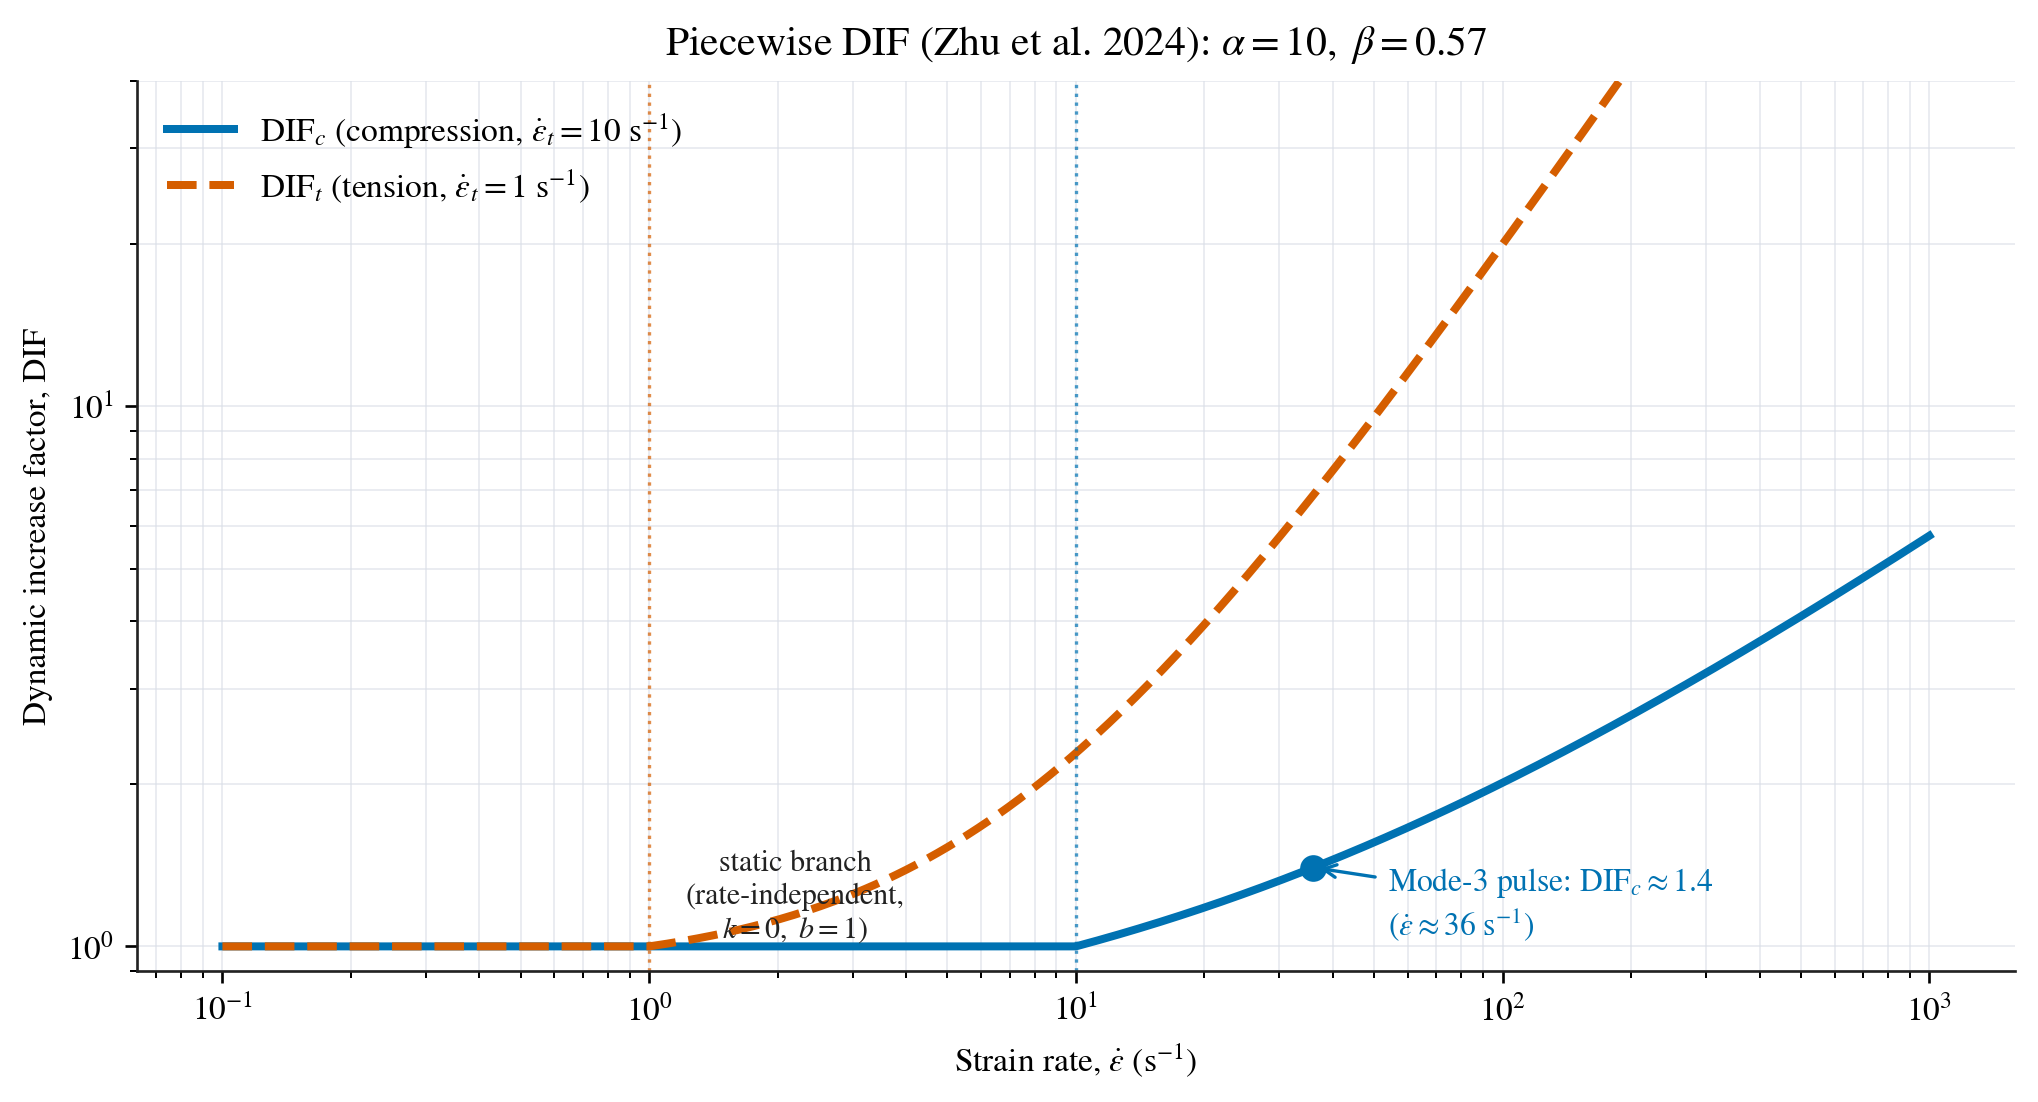
\includegraphics[width=\linewidth]{trihb_dif.png}
    \caption{Dynamic increase factor}
  \end{subfigure}
  \caption{True-triaxial and rate-dependent failure envelope. (a) The default
  Lode and Willam--Warnke shapes correctly weaken the extension meridian relative
  to compression ($\rho_t/\rho_c=0.70$), capturing the $\sigma_2$ effect; the
  legacy cap (dotted) has the opposite, unphysical sense. (b) Piecewise dynamic
  increase factor of~\citet{ZHU2024105948} (Eqs.~\eqref{eq:difc}--\eqref{eq:dift}):
  a rate-independent static branch ($\mathrm{DIF}=1$) below the transition rate
  ($10~\mathrm{s^{-1}}$ in compression, $1~\mathrm{s^{-1}}$ in tension) and a
  power-law dynamic branch above it ($\alpha=10$, $\beta=0.57$); $\mathrm{DIF}_t$
  rises faster ($\propto\dot\varepsilon^{2\beta}$) than $\mathrm{DIF}_c$
  ($\propto\dot\varepsilon^{\beta}$). The Mode-3 pulse
  ($\dot\varepsilon\approx36~\mathrm{s^{-1}}$) gives $\mathrm{DIF}_c\approx1.4$.}
  \label{fig:envelope}
\end{figure}

\subsection{True-triaxial criteria: Mogi--Coulomb and modified Lade}\label{sec:criteria}

The one-parameter Lode shape is a first-order surrogate; for studies that target
the intermediate principal stress the workspace offers two calibrated
true-triaxial criteria, both derived from the \emph{same} unconfined strength and
confinement ratio so all three surfaces are directly comparable. The
\emph{Mogi--Coulomb} criterion~\citep{mogi1971,alajmi2005} sets the octahedral
shear against the mean of the extreme principal stresses,
\begin{equation}
\tau_{\mathrm{oct}}=a+b\,\sigma_{m,2},\qquad
\sigma_{m,2}=\tfrac12(\sigma_1+\sigma_3),\qquad
\tau_{\mathrm{oct}}=\tfrac{\sqrt2}{3}\,q\ \ (\text{Eq.~\eqref{eq:invariants}}),
\label{eq:mogi}
\end{equation}
with $a=\tfrac{2\sqrt2}{3}c\cos\phi$ and $b=\tfrac{2\sqrt2}{3}\sin\phi$ from the
Coulomb cohesion and friction angle implied by the strength data,
$\sin\phi=(k_{\mathrm{conf}}-1)/(k_{\mathrm{conf}}+1)$ and
$c=\mathrm{UCS}\,(1-\sin\phi)/(2\cos\phi)$. Although $\sigma_{m,2}$ omits
$\sigma_2$, the octahedral shear $\tau_{\mathrm{oct}}$ retains it, so the criterion
is $\sigma_2$-dependent. The \emph{modified Lade} criterion~\citep{ewy1999} uses
the smooth, corner-free form
\begin{equation}
\frac{I_1''^{\,3}}{I_3''}=27+\eta,\qquad
I_1''=\textstyle\sum_i(\sigma_i+S),\quad I_3''=\textstyle\prod_i(\sigma_i+S),\quad
S=\frac{c}{\tan\phi},\quad
\eta=\frac{4\tan^2\phi\,(9-7\sin\phi)}{1-\sin\phi},
\label{eq:lade}
\end{equation}
the translation $S$ shifting the apex to embed the tensile strength. By
construction both reduce to $\sigma_1=\mathrm{UCS}$ when unconfined and to the
Coulomb meridian $\sigma_1=\mathrm{UCS}+k_{\mathrm{conf}}\sigma_3$ in triaxial
compression ($\sigma_2=\sigma_3$). Two further $\sigma_2$-sensitive surfaces are
provided. \emph{Yu's unified strength theory}~\citep{yu2002} is the piecewise
twin-shear form
\begin{equation}
\max\!\Big[\sigma_1-\tfrac{k_{\mathrm{conf}}}{1+b}(b\sigma_2+\sigma_3),\ \
\tfrac{1}{1+b}(\sigma_1+b\sigma_2)-k_{\mathrm{conf}}\sigma_3\Big]=\mathrm{UCS},
\label{eq:yu}
\end{equation}
whose unified parameter $b\in[0,1]$ interpolates from Mohr--Coulomb ($b=0$) to the
twin-shear bound ($b=1$); the two linear branches switch at
$\sigma_2=(\sigma_1+k_{\mathrm{conf}}\sigma_3)/(k_{\mathrm{conf}}+1)$, producing
the $\sigma_2$ enhancement. The \emph{modified Wiebols--Cook}
criterion~\citep{wiebols1968} is the smooth quadratic
\begin{equation}
\sqrt{J_2}=A_w+B_w J_1+C_w J_1^{2},\qquad J_1=\sigma_1+\sigma_2+\sigma_3,
\label{eq:wc}
\end{equation}
with $A_w,B_w,C_w$ fixed by the unconfined strength and the triaxial-compression
meridian; here the $\sigma_2$-dependence enters through $J_1$ and $J_2$. Polyaxial
benchmarking finds such $\sigma_2$-sensitive criteria outperform
$\sigma_2$-independent ones for rock~\citep{colmenares2002}.

The five surfaces differ in \emph{how} strongly the intermediate stress
strengthens the rock. To reflect a realistic test, Figure~\ref{fig:criteria}a uses
the \emph{dynamic} strength --- the quasi-static surface inflated by a
representative rate factor $\mathrm{DIF}_c\approx1.4$ (Eq.~\eqref{eq:difc} at
$\dot\varepsilon\approx36~\mathrm{s^{-1}}$), consistent with the
multi-impact tests~\citep{wang2022progressive} --- and treats the principal
stresses as \emph{total}. The static pre-stress is capped at $\sim\!\SI{50}{MPa}$
by the hydraulic confinement, so the intermediate stress can only exceed
$\SI{50}{MPa}$ through the \emph{dynamic confinement} the impact develops on the
lateral bars ($\sigma_2,\sigma_3=\sigma_{\mathrm{pre}}+\Delta\sigma_{\mathrm{dyn}}$);
this is why the dynamic strengths $\sigma_1$ reach several hundred MPa rather than
the quasi-static values. At $\sigma_3=\SI{50}{MPa}$ the classical
($\sigma_2$-blind) Mohr--Coulomb strength is flat at
$\sigma_1=\mathrm{UCS}\!\cdot\!\mathrm{DIF}+k_{\mathrm{conf}}\sigma_3$, whereas
every $\sigma_2$-aware surface rises with $\sigma_2$ across the physically
accessible range --- the intermediate-stress strengthening~\citep{mogi1971} --- the
five spreading by $\sim\!15$--$20\%$ at the upper end and all coinciding on the
triaxial-compression ($\sigma_2=\sigma_3$) Coulomb line by construction. Evaluated
along the Tri-HB Mode-3 stress path of Fig.~\ref{fig:stresspath}
(Fig.~\ref{fig:criteria}b), the criteria report different peak failure indices for
the \emph{same} loading ($F_{\max}\approx1.1$--$1.5$), so the choice of surface
materially changes the predicted dynamic strength. Which surface is correct for a
given rock is an experimental question --- precisely the $\sigma_2$-resolved
measurement the Tri-HB provides --- after which the meridian, the Lode ratio and
the criterion are fitted to the data.

\begin{figure}[t]
  \centering
  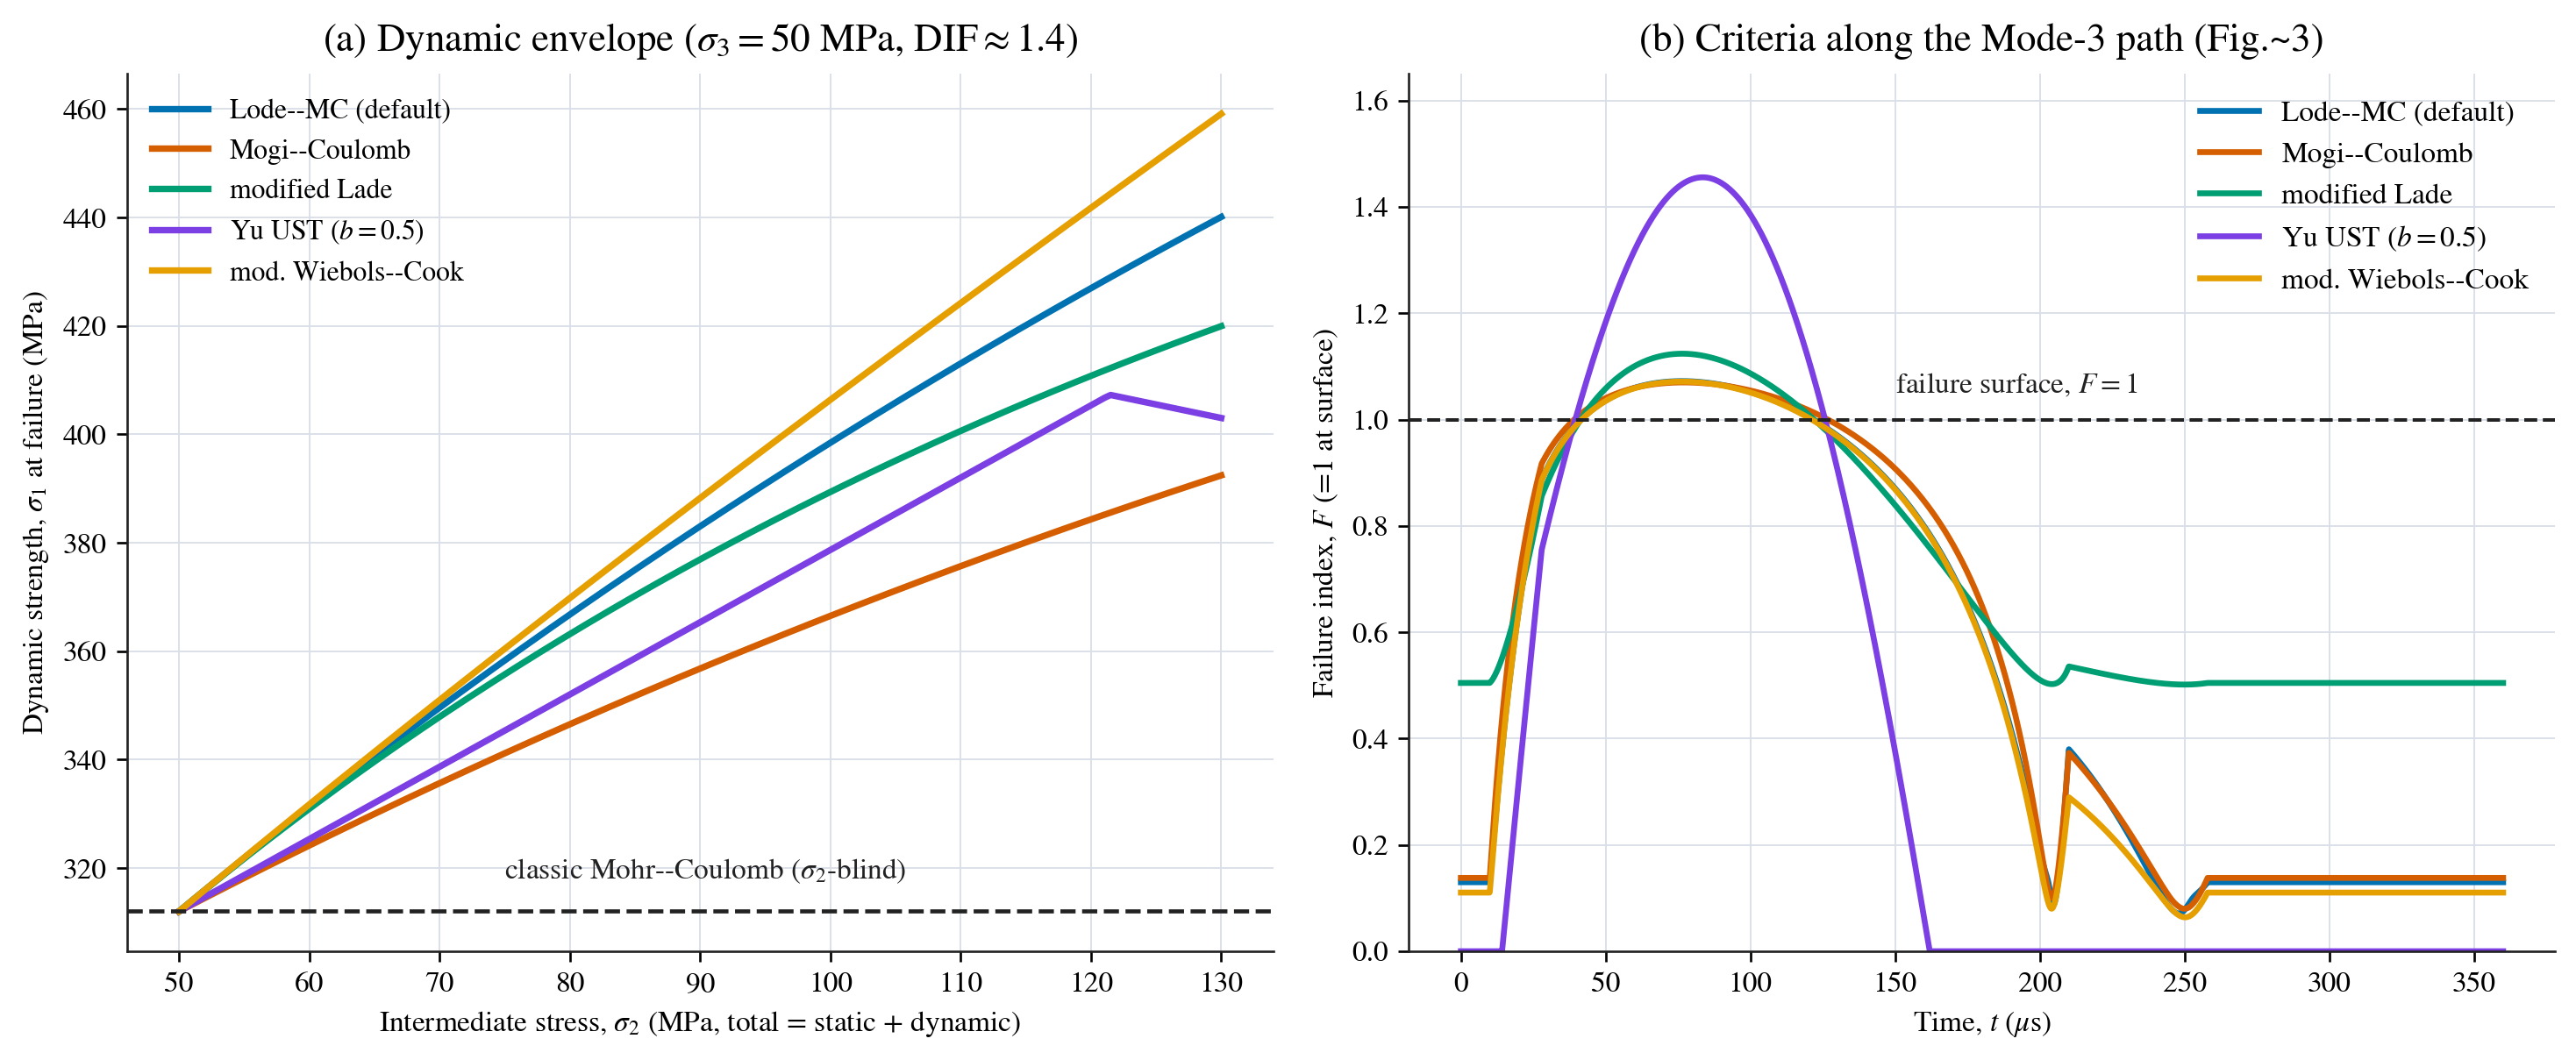
\includegraphics[width=\linewidth]{trihb_criteria_comparison.png}
  \caption{True-triaxial failure criteria at realistic Tri-HB conditions, all
  calibrated to the same dynamic strength ($\mathrm{UCS}\!\cdot\!\mathrm{DIF}$,
  $\mathrm{DIF}\approx1.4$) and $k_{\mathrm{conf}}=4$. (a) Failure strength
  $\sigma_1$ versus the \emph{total} intermediate stress $\sigma_2$ at
  $\sigma_3=\SI{50}{MPa}$: the classical Mohr--Coulomb surface is $\sigma_2$-blind
  (flat), while the Lode--MC, Mogi--Coulomb, modified-Lade, Yu-UST and modified
  Wiebols--Cook surfaces capture the intermediate-stress strengthening; $\sigma_2$
  exceeds the $\SI{50}{MPa}$ static cap only through dynamic confinement. (b) The
  corresponding failure indices ($F=1$ at the surface) along the Tri-HB Mode-3
  stress path of Fig.~\ref{fig:stresspath}.}
  \label{fig:criteria}
\end{figure}

\subsection{Energy-consistent damage dissipation}\label{sec:energy}

Damage $D$ evolves by a Perzyna-type overstress law with load-shedding feedback,
\begin{equation}
\dot D=\frac{(1-D)^{\alpha}}{\tau_D}
\Big\langle\frac{F_{\mathrm{eff}}-1}{F_0}\Big\rangle^{m}
\Big(\frac{|\epsd_{\mathrm{eq}}|}{\epsd_0}\Big)^{\beta},
\qquad F_{\mathrm{eff}}=(1-D)\,F,
\label{eq:damage}
\end{equation}
where $\langle\cdot\rangle$ is the Macaulay bracket and
$\tau_D,\alpha,m,\beta,F_0,\epsd_0$ are kinetic constants. The load-shedding
factor $F_{\mathrm{eff}}=(1-D)\,F$ is the key feature: as $D$ grows, the effective
overstress $\langle F_{\mathrm{eff}}-1\rangle$ shrinks and the growth rate decays,
so $D$ approaches a finite steady value rather than diverging to
unity~\citep{perzyna1966,lemaitre1985}. The energy partition is, moreover, now
derived from this single constitutive relation. Damage degrades the secant modulus to $E_0(1-D)$, so the specimen
carries the damage-coupled elastic strain and the work, recoverable energy and
dissipation become
\begin{equation}
\varepsilon_i=\frac{\sigma_i-\nu(\sigma_j+\sigma_k)}{E_0(1-D)},\quad
W_{\mathrm{input}}=\!\int_0^t\!\sigma_i\dot\varepsilon_i\,\mathrm{d}\tau,\quad
W_{\mathrm{el}}=\tfrac12\sigma_i\varepsilon_i,\quad
W_{\mathrm{diss}}=\big\langle W_{\mathrm{input}}-W_{\mathrm{el}}\big\rangle .
\label{eq:energy}
\end{equation}
The first law then closes by construction,
$W_{\mathrm{input}}=W_{\mathrm{el}}+W_{\mathrm{diss}}$: the input work ends above
zero by exactly the dissipated part, the recoverable energy returns toward zero on
unloading, and the dissipation rises monotonically (Fig.~\ref{fig:energy}). This
removes the inconsistency of treating the input work as fully recoverable while
estimating dissipation from a separate integral. The partition is non-negative by
construction, $W_{\mathrm{diss}}=\langle W_{\mathrm{input}}-W_{\mathrm{el}}\rangle\ge0$,
and monotone in all reference cases (Fig.~\ref{fig:energy}); we therefore call it
\emph{energetically self-consistent} rather than claiming full thermodynamic
admissibility, for which a pointwise dissipation inequality
$\dot W_{\mathrm{diss}}\ge0$ from a Clausius--Duhem argument with the free energy
remains future work. Equation~\eqref{eq:energy} is, furthermore, the
\emph{scalar}-damage partition; the orthotropic model of \S\ref{sec:ortho} is a
first-stage extension that still inherits it through $D=\max_i D_i$, with the
fully anisotropic form --- $W_{\mathrm{el}}$ built from a damaged compliance
tensor $\mathbf{S}(\mathbf{D})$ rather than a scalar secant modulus --- also left
to future work.

\begin{figure}[t]
  \centering
  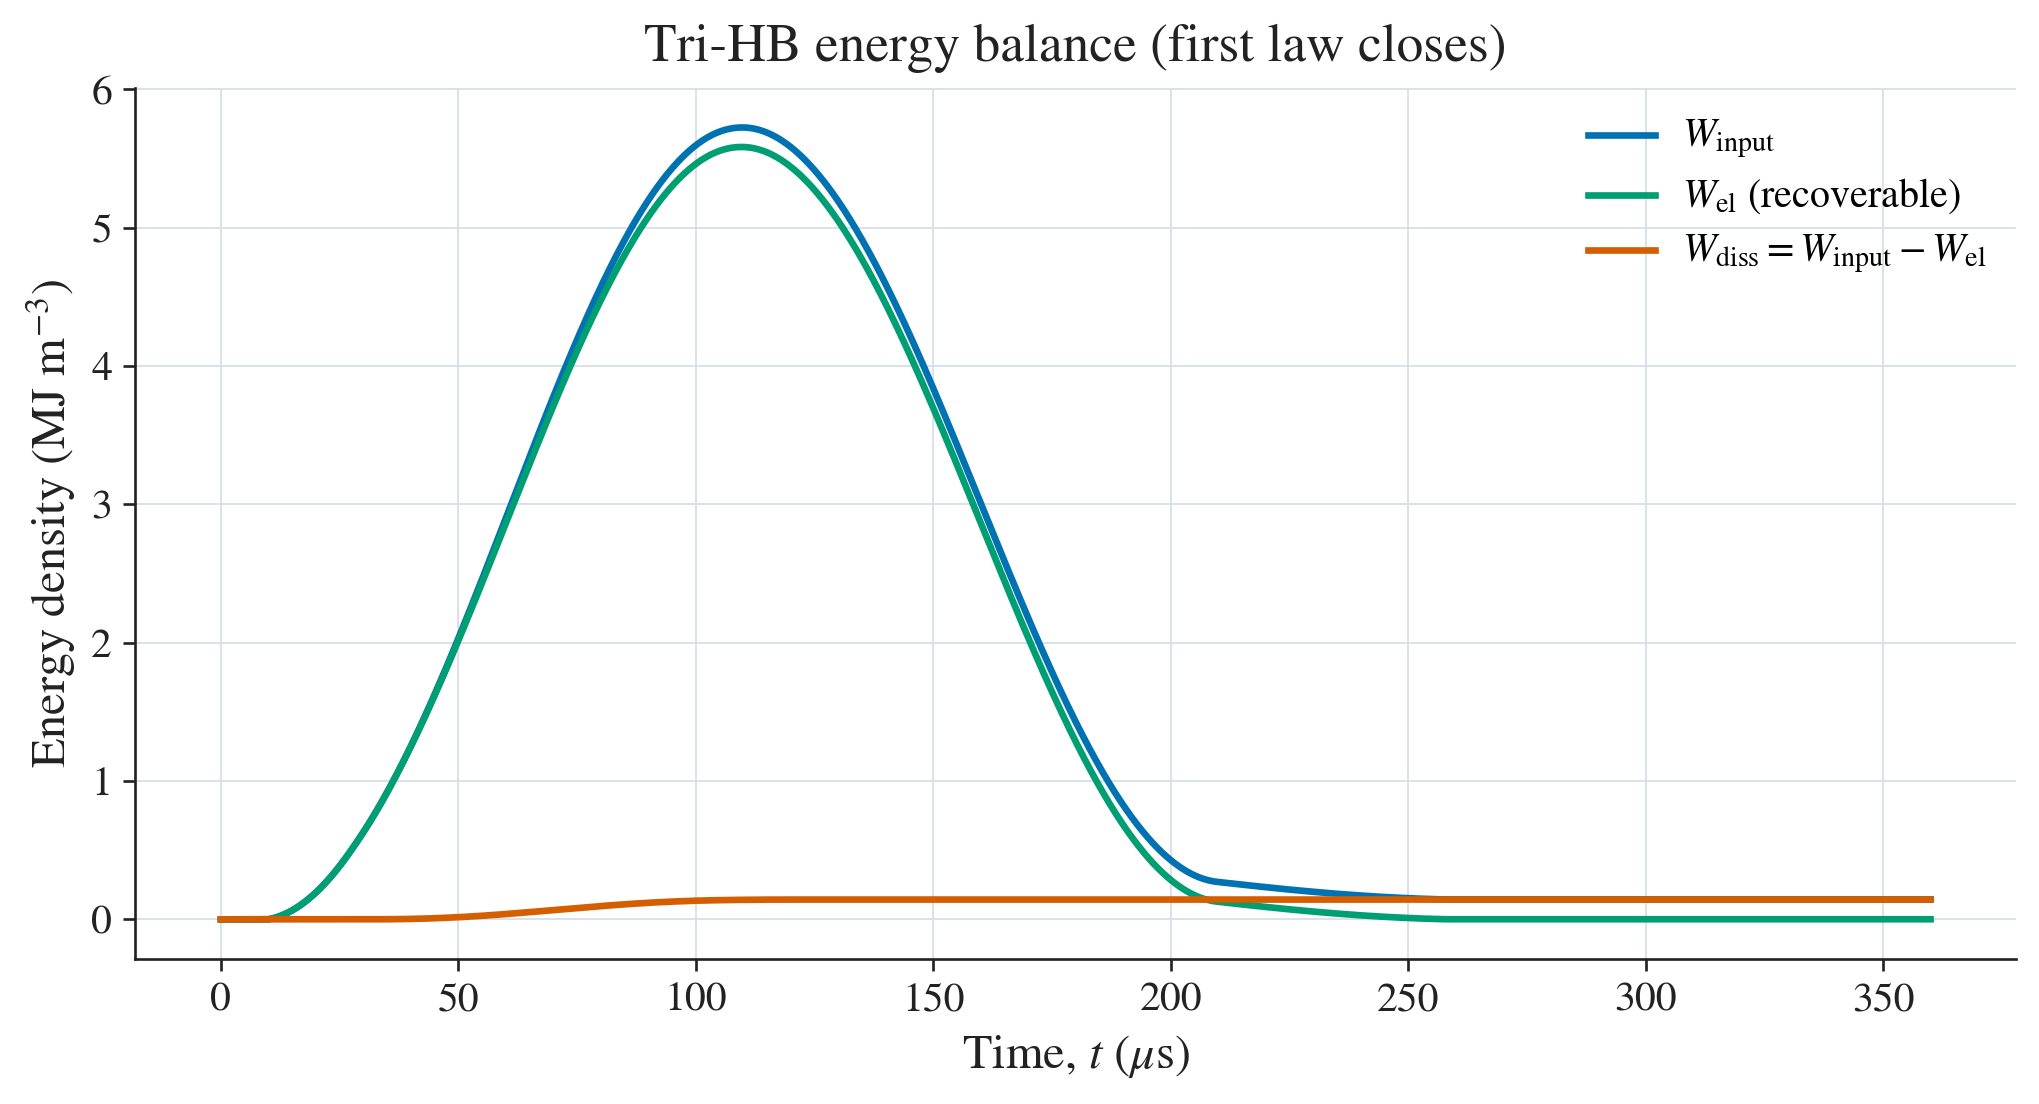
\includegraphics[width=0.62\linewidth]{trihb_energy.png}
  \caption{Energy-density partition (Step~4) for the gas-gun Tri-HB case. With the damage-coupled strain the
  balance closes exactly: $W_{\mathrm{input}}=W_{\mathrm{el}}+W_{\mathrm{diss}}$,
  with $W_{\mathrm{diss}}$ the non-recoverable (dissipated) energy.}
  \label{fig:energy}
\end{figure}

\subsection{Orthotropic damage for blasting-induced fracturing}\label{sec:ortho}

Rock blasting produces \emph{directional} fracture: radial cracks and spall open
perpendicular to the local tension, so the stiffness and wave-speed loss differ
by direction. A scalar $D$ cannot represent this. The Tri-HB computational workspace
therefore offers a diagonal damage tensor $\mathbf{D}=\mathrm{diag}(D_x,D_y,D_z)$
aligned with the bars. Each component evolves through the same overstress kinetics,
driven by a \emph{dominant directional-tensile} term plus a \emph{small
shear/compaction} term,
\begin{equation}
\dot D_i=\frac{(1-D_i)^{\alpha}}{\tau_D}
\Big\langle\frac{(1-D_i)F_i-1}{F_0}\Big\rangle^{m}
\Big(\frac{|\epsd_{\mathrm{eq}}|}{\epsd_0}\Big)^{\beta},\qquad
F_i=\frac{\langle-\varepsilon_i\rangle_+}{\varepsilon_{t0}}
+\kappa_s\Big\langle\frac{F-F_{s0}}{1-F_{s0}}\Big\rangle,
\label{eq:ortho}
\end{equation}
for $i=x,y,z$, with $\varepsilon_{t0}=\sigma_t/E_0$ ($\sigma_t$ the tensile
strength), $F=q/q_f$ the deviatoric failure index of \S\ref{sec:env}, and
$(\kappa_s,F_{s0})=(1,0.5)$ here. The first term is \emph{tensile}: in the
compression-positive convention a tensile strain is negative, so
$\langle-\varepsilon_i\rangle_+=\max(-\varepsilon_i,0)$ extracts the extensile
strain that opens cracks on the plane normal to axis $i$. The second term is an
\emph{isotropic} shear/compaction contribution that switches on once the
deviatoric index exceeds $F_{s0}$; it represents the wing-crack, shear-microcrack
and grain-crushing damage that real rock accrues \emph{even under net
compression}. Because $F$ only modestly exceeds unity at the dynamic peak
($F_{\max}\!\approx\!1.14$ here), this term accrues only a small axial damage,
whereas the tensile term --- fed by the large lateral extensile strains ---
dominates the lateral axes. Axial $X$ compression therefore drives large lateral
components $D_y,D_z$ (axial splitting) while giving a \emph{small but nonzero}
axial component $D_x\!\ll\!D_y,D_z$ (here $D_x\!\approx\!0.1$ versus
$D_y\!\approx\!0.75$, $D_z\!\approx\!0.83$) --- consistent with the modest
axial-stiffness loss seen in dynamically compressed rock, rather than the
unphysical $D_x\!=\!0$ of a pure-tension model. Confinement on an axis suppresses
its tensile damage, so the least-confined lateral axis ($Z$) is the most damaged
(Fig.~\ref{fig:ortho}a). The per-axis modulus
degrades independently, $E_i=E_0(1-D_i)$ (Fig.~\ref{fig:ortho}b), as does the
directional wave speed $c_{p,i}=c_{p0}\sqrt{1-D_i}$. This formulation is rooted
in the microcrack-damage tradition for brittle rock~\citep{grady1980,taylor1986}
but resolves damage by direction. Decisively, because the three orthogonal bars
measure direction-resolved modulus and wave-speed loss, each $D_i$ can be
calibrated \emph{component-by-component} from a single true-triaxial test --- a
measurement a uniaxial SHPB cannot provide.

\begin{figure}[t]
  \centering
  \begin{subfigure}[b]{0.49\linewidth}
    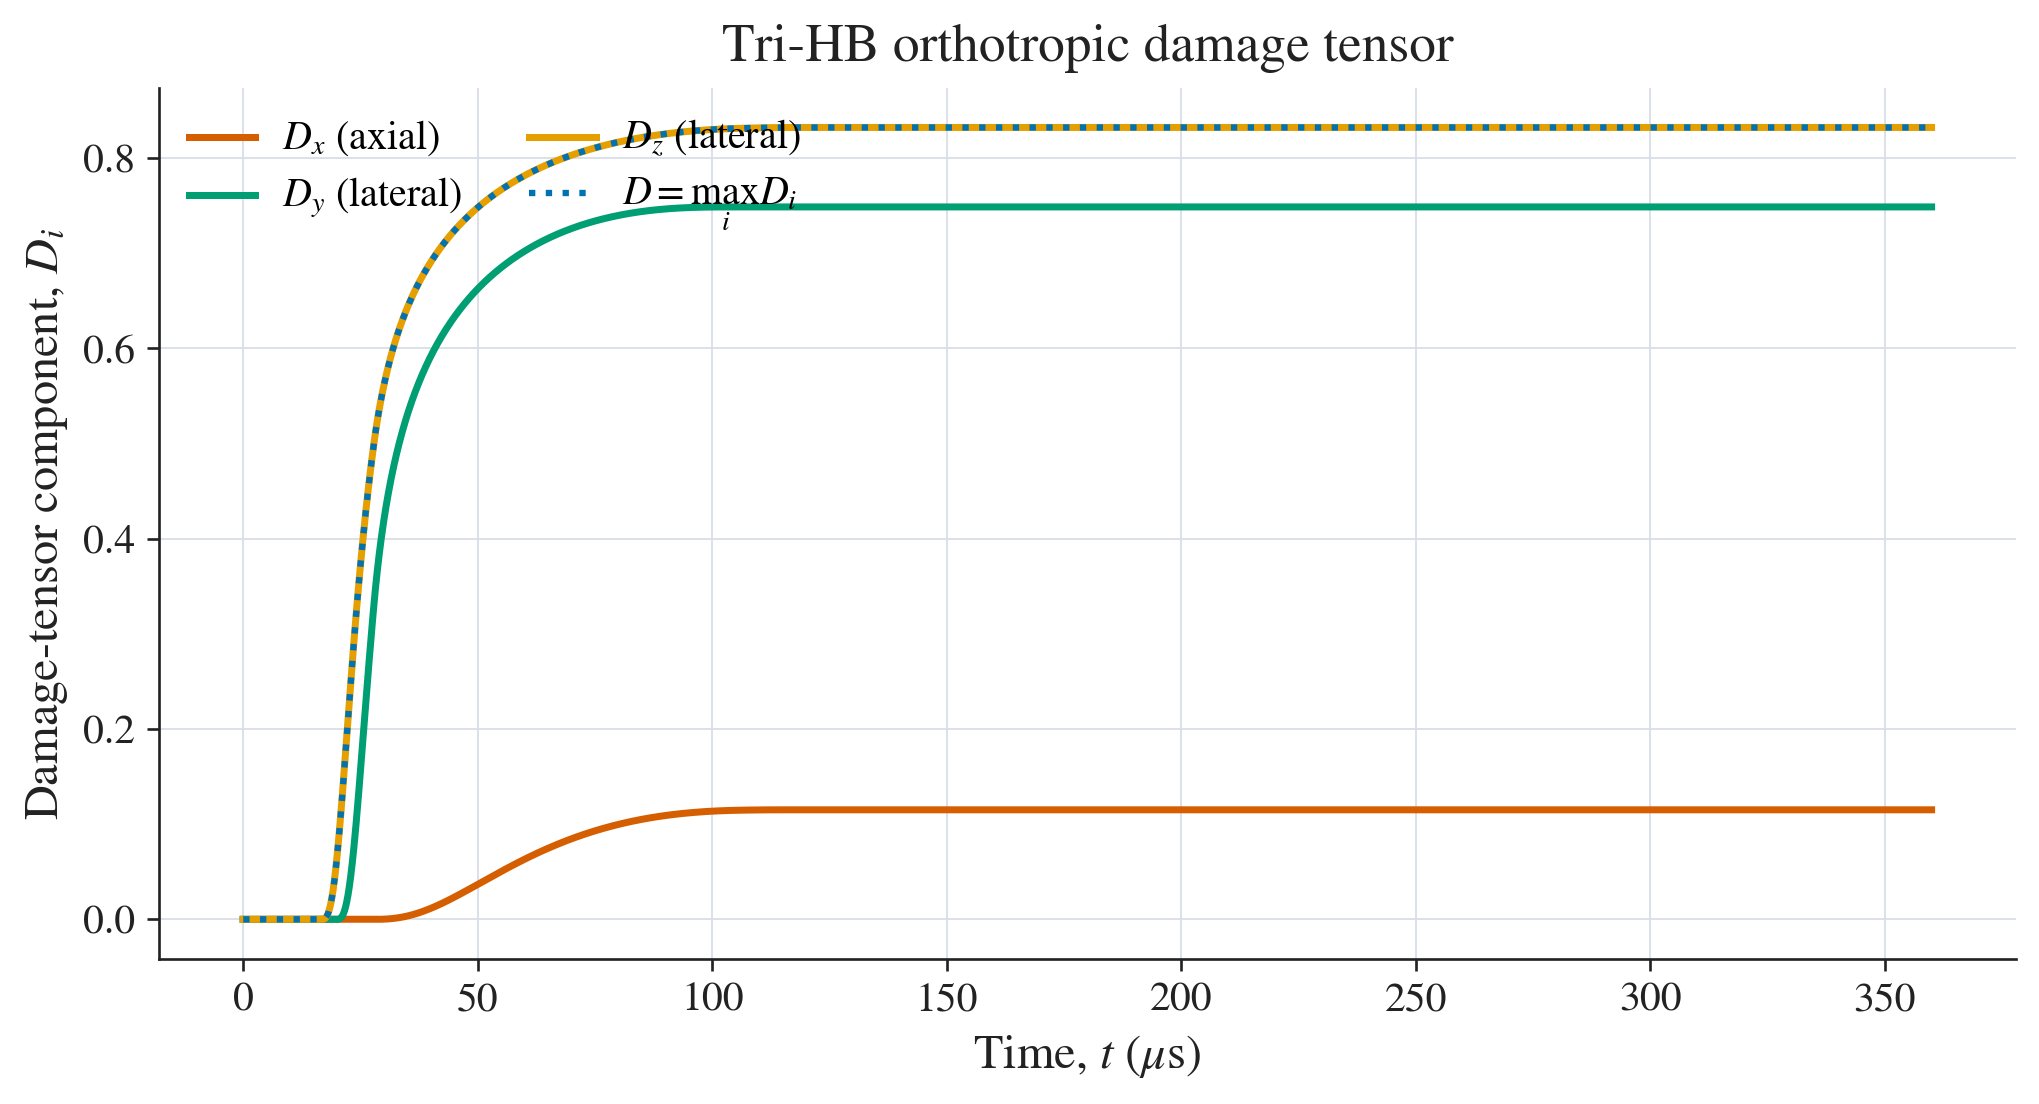
\includegraphics[width=\linewidth]{trihb_orthotropic_damage.png}
    \caption{Damage-tensor components $D_x,D_y,D_z$}
  \end{subfigure}\hfill
  \begin{subfigure}[b]{0.49\linewidth}
    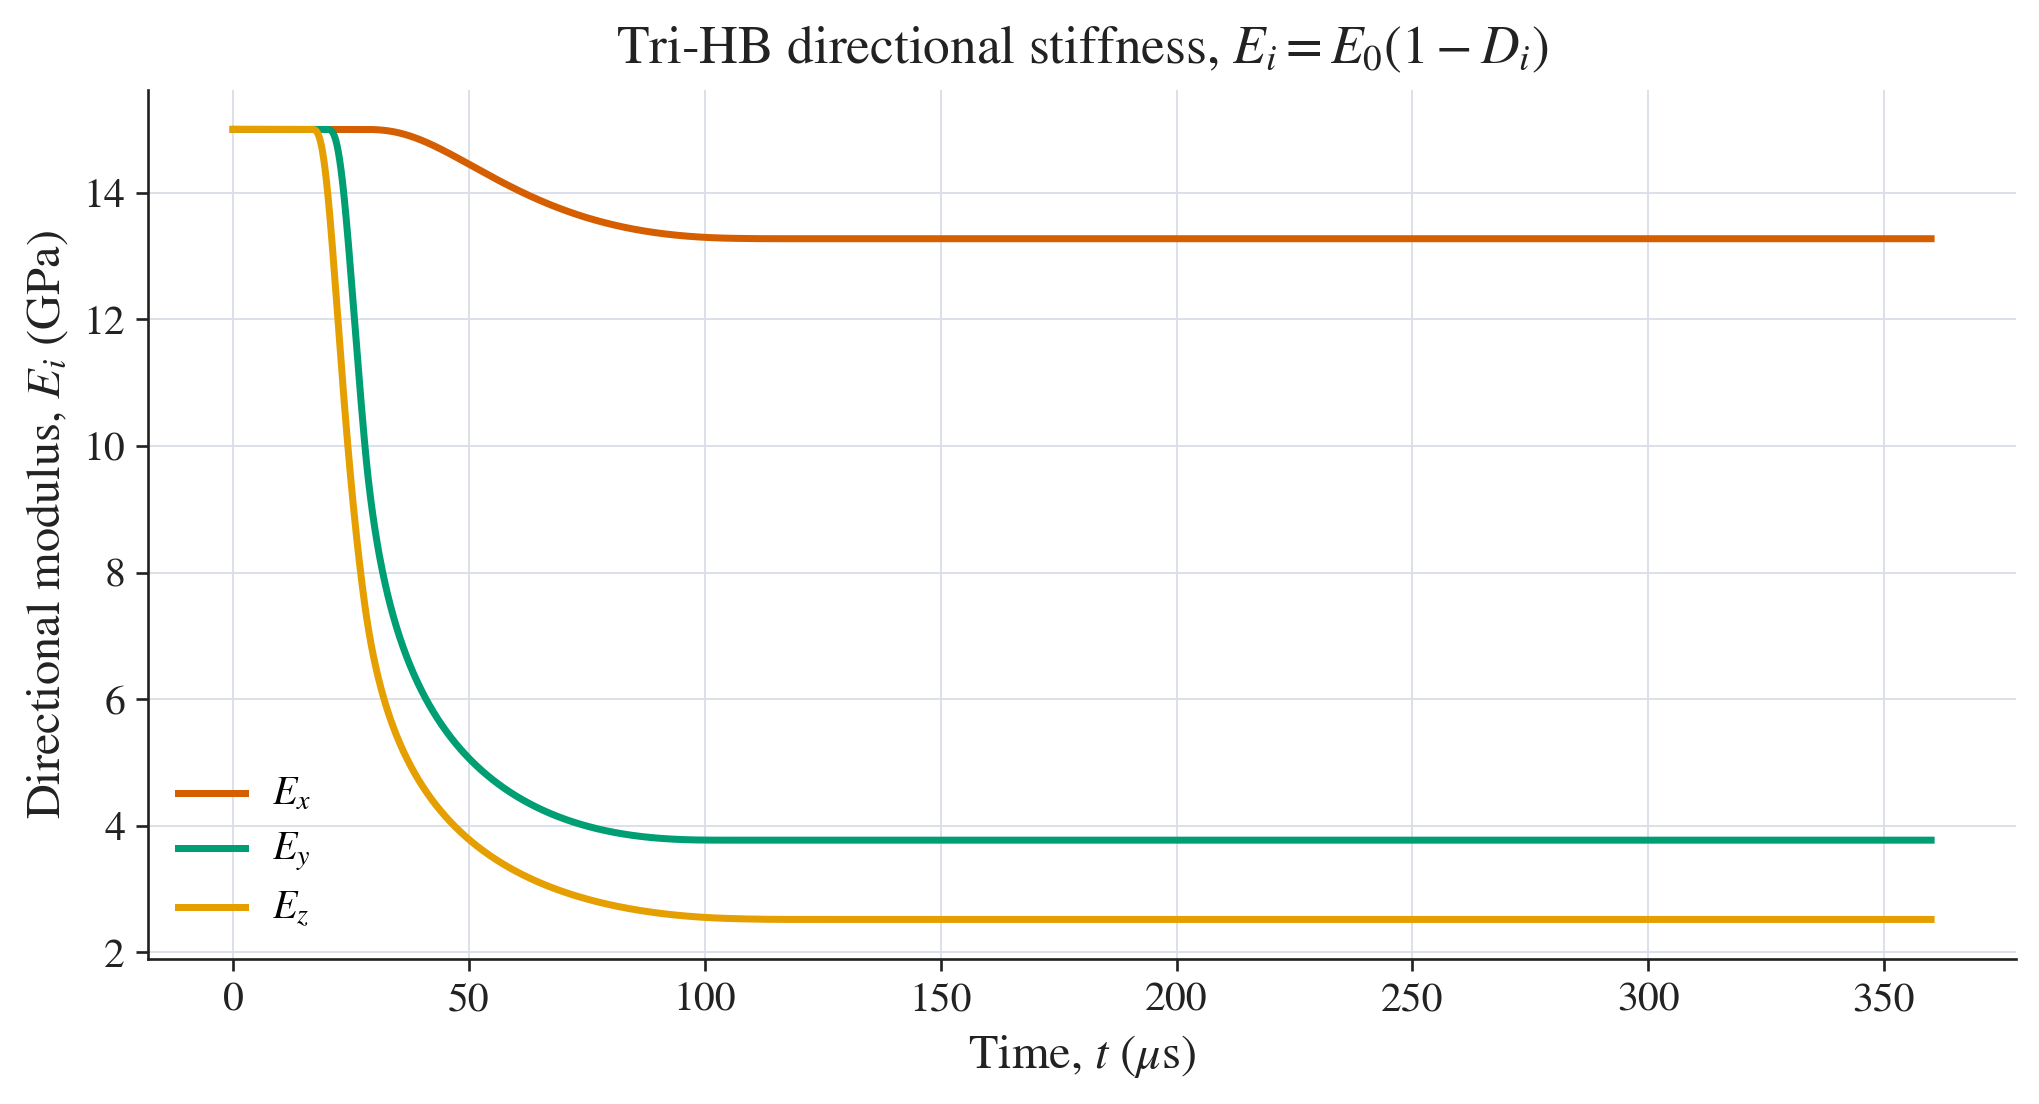
\includegraphics[width=\linewidth]{trihb_directional_stiffness.png}
    \caption{Directional stiffness $E_i=E_0(1-D_i)$}
  \end{subfigure}
  \caption{Orthotropic (Stage-1) damage for the gas-gun Tri-HB (Mode~3) case. (a) The
  diagonal damage-tensor components: a dominant tensile driver gives large lateral
  damage ($D_z\!>\!D_y$, the least-confined axis most damaged), while a small
  shear/compaction driver gives a nonzero but much smaller axial $D_x\!\approx\!0.1$;
  the scalar $D=\max_i D_i$ governs the energy/stiffness summary. (b) The resulting
  directional modulus loss: $E_x$ falls modestly while $E_y,E_z$ fall sharply ---
  the per-axis quantity the three bar pairs measure.}
  \label{fig:ortho}
\end{figure}

\subsection{Cyclic dynamic loading and cumulative damage}\label{sec:cyclic}

Because each axis is loaded through bars rather than a sealed chamber, the Tri-HB
can hold the specimen at its in-situ static pre-stress, fire one dynamic pulse,
reset to the same static state, and re-fire the \emph{same} pulse --- repeating
until the rock fails. This reproduces repeated blasting, repeated rockburst
loading and dynamic fatigue of a pre-stressed rock mass~\citep{wang2022progressive}, none of which a
single-shot SHPB can access. At the high amplitudes used in practice the rock
fails within a few impacts (typically $N_f\!\lesssim\!10$); tens or hundreds of
impacts are neither feasible nor observed.

Damage carries over between impacts and degrades the strength
$q_f(D)=q_{f,0}(1-D)^{c_d}$, so an impact the rock survives once accumulates to
failure~\citep{ZHU2024105948}. With impact index $k$ and the failure index $F=q/q_f$ from the active
criterion (Lode, Mogi--Coulomb or modified Lade), the cumulative-damage map is
\begin{equation}
\begin{aligned}
D_k&=\min(D_{k-1}+\Delta D_k,1),\qquad F_k=F_1(1-D_{k-1})^{-c_d},\\
\Delta D_k&=K\big\langle(1-D_{k-1})F_k-F_{\mathrm{th}}\big\rangle^{m}(1-D_{k-1})^{\alpha},
\end{aligned}
\label{eq:cyclic}
\end{equation}
which keeps the same Perzyna kinetics~\citep{perzyna1966,lemaitre1985} integrated
over one pulse --- appropriate because repeated impact is \emph{low-cycle}
($N\!\lesssim\!20$) fatigue, in which each high-amplitude impact is a genuine
overstress excursion. The effective driving $(1-D)F_k=F_1(1-D)^{1-c_d}$ exposes
three regimes through the exponent $1-c_d$: shakedown ($c_d<1$), linear
Palmgren--Miner accumulation ($c_d=1$), and accelerating progressive failure
($c_d>1$). The last is \emph{abrupt}: the strength-degradation feedback produces a
sharp sigmoid that cascades to failure once the degraded strength is first
exceeded, at the critical damage $D^\ast=1-F_1^{1/c_d}$ --- reproducing the sudden
damage threshold seen in synchrotron micro-CT of multi-impact tests~\citep{wang2022progressive}
(Fig.~\ref{fig:cyclic}).

\begin{figure}[t]
  \centering
  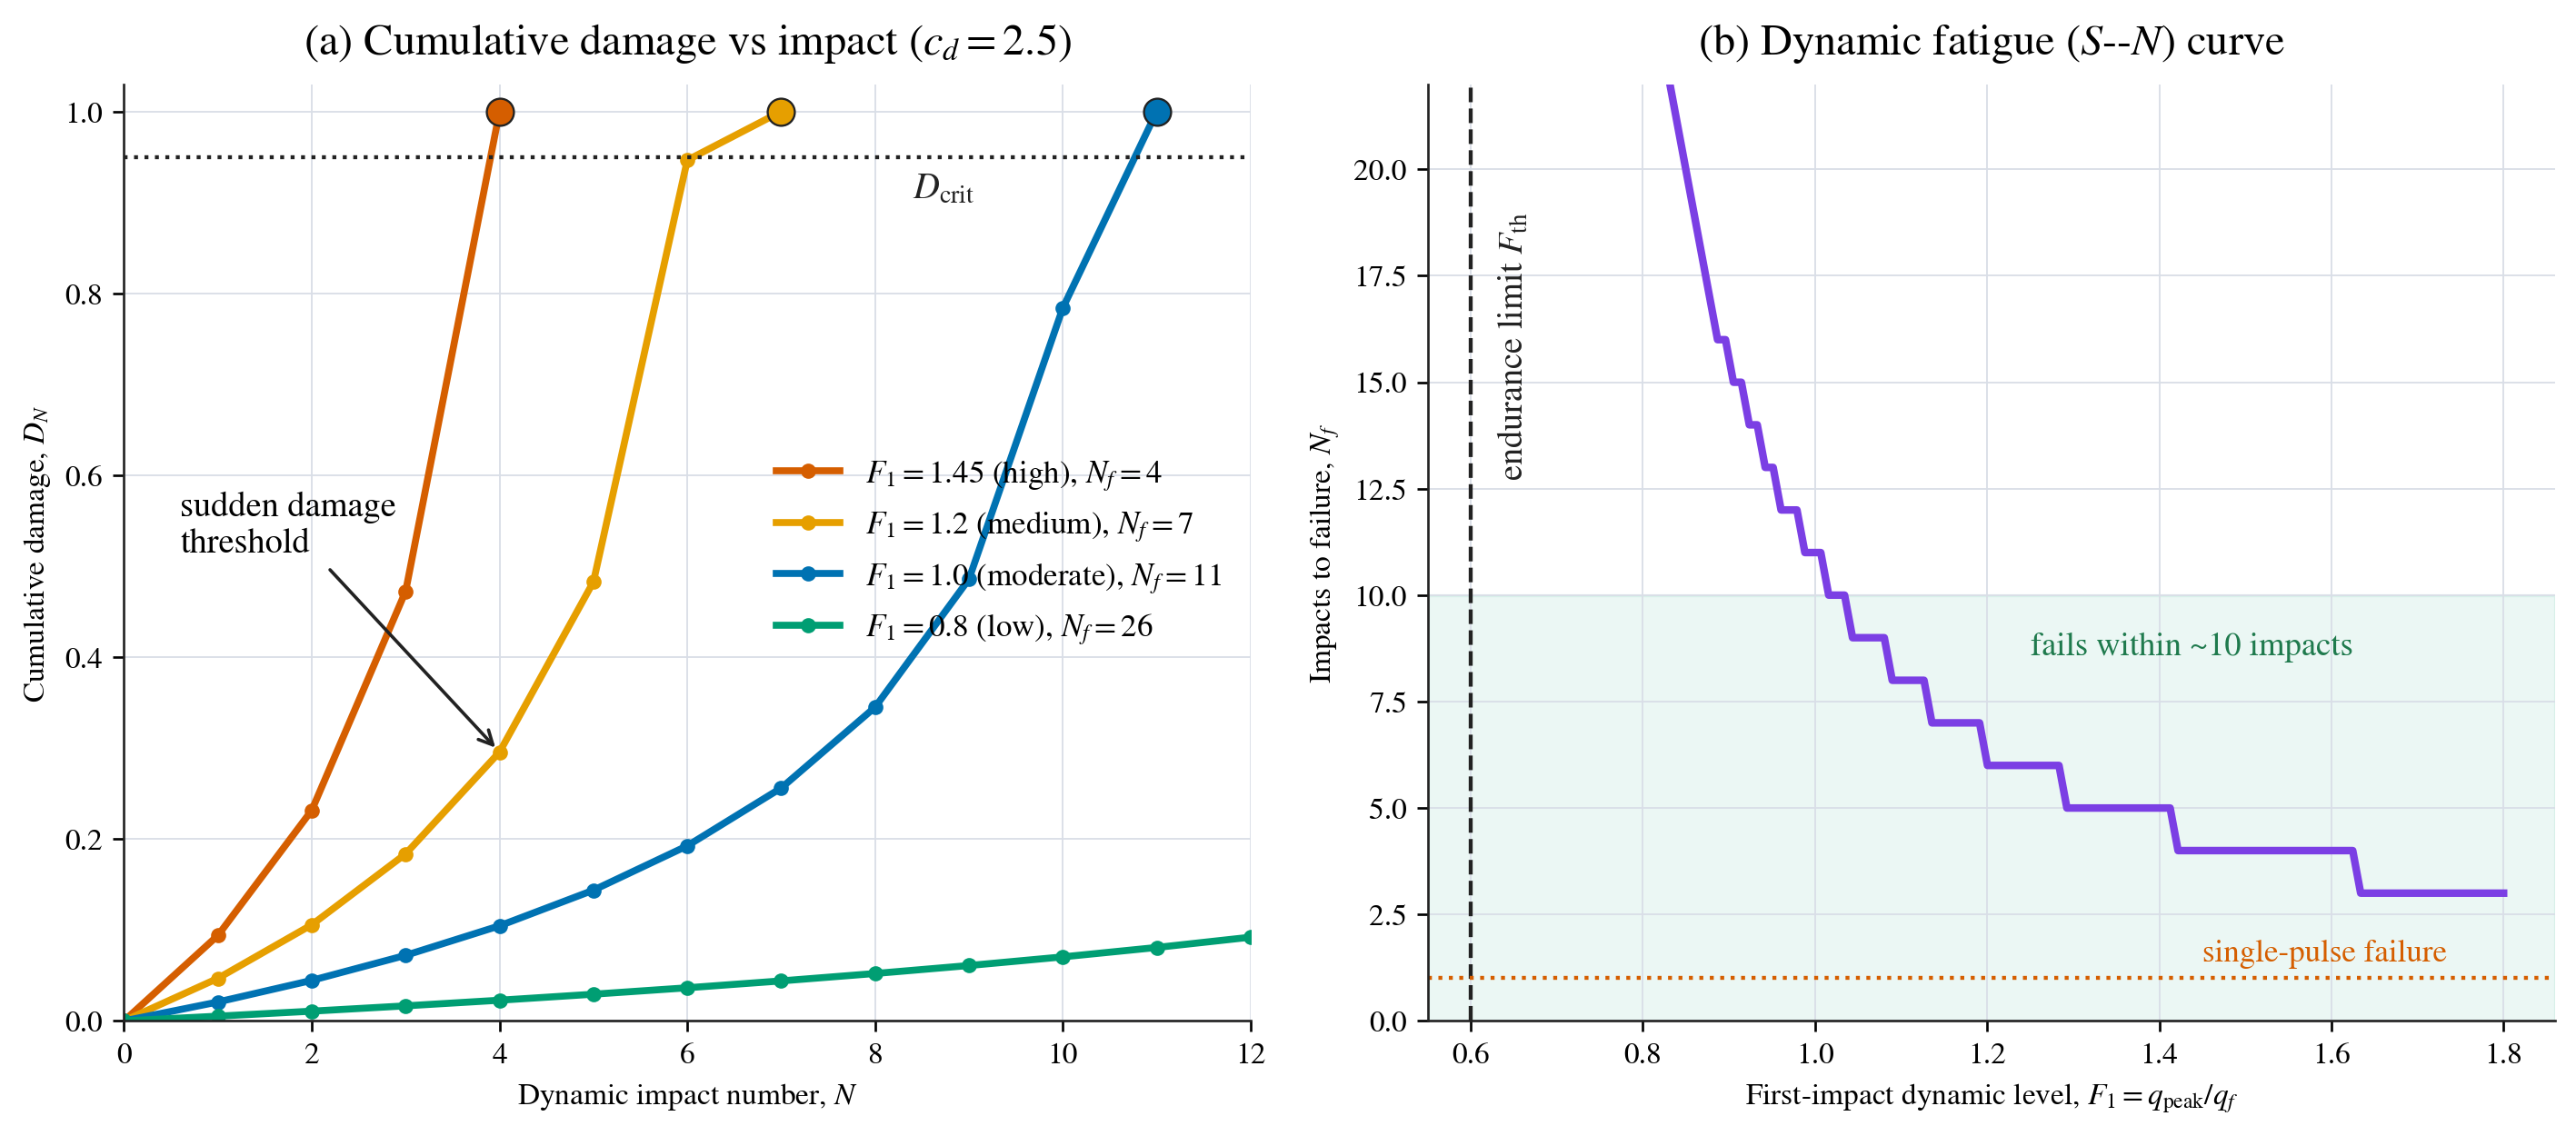
\includegraphics[width=\linewidth]{trihb_cyclic_damage.png}
  \caption{Cyclic (repeated) dynamic loading. (a) Cumulative damage versus impact
  number: high levels fail the rock within a few impacts through a sudden
  threshold (sharp sigmoid), low levels need impractically many. (b) The
  dynamic-fatigue ($S$--$N$) curve --- impacts-to-failure fall into the realistic
  $\lesssim\!10$ band at high level and diverge at the endurance limit
  $F_{\mathrm{th}}$.}
  \label{fig:cyclic}
\end{figure}

Equation~\eqref{eq:cyclic} is the spatially uniform reduction of a two-scale
field problem. The fast intra-impact wave IBVP couples the wave equation to the
local damage rate,
\begin{equation}
\rho\,\partial_{tt}u=\partial_x\!\big[E_0(1-D)\,\partial_x u\big],\qquad
\partial_t D=\frac{(1-D)^{\alpha}}{\tau_D}\Big\langle\tfrac{(1-D)F-1}{F_0}\Big\rangle^{m}\Big(\tfrac{|\dot\varepsilon_{\mathrm{eq}}|}{\dot\varepsilon_0}\Big)^{\beta},
\label{eq:cyclic-ibvp}
\end{equation}
with the \emph{inherited} damage field $D(x,0)=D_{k-1}(x)$ as initial condition,
so the bar coefficients $E_0(1-D)$, $c_p$ and $Z$ become evolving heterogeneous
fields. Averaging over one pulse gives the slow inter-impact drift
$\partial_N D=\int_0^{T_p}\partial_t D\,\mathrm{d}\tau$; because the degraded
strength softens, the local form is ill-posed and is regularised by a gradient
(nonlocal) term with internal length $\ell$~\citep{pijaudier1987},
\begin{equation}
\frac{\partial D}{\partial N}=\frac{1}{\tau_N}\big\langle(1-D)\,\bar F-F_{\mathrm{th}}\big\rangle^{m}(1-D)^{\alpha},
\qquad \bar D=D-\ell^2\nabla^2 D,
\label{eq:cyclic-bvp}
\end{equation}
with $\nabla D\cdot\mathbf{n}=0$ on $\partial\Omega$; $\ell$ sets the
fracture-band width. The per-impact damage is independently measurable: the
soft-recovered specimen is micro-CT scanned after each impact, and the directional
crack-density tensor gives $D_i=1-E_i/E_0$ to compare against the predicted $D_k$,
so $\ell$, $\tau_N$ and $c_d$ are calibrated from the measured
damage-versus-impact trajectory and the locus of per-impact peak stresses recovers
the monotonic post-peak envelope.

\subsection{Spatial damage verification: gradient field and phase-field}\label{sec:spatial}

The two-scale formulation of \S\ref{sec:cyclic}
(Eqs.~\eqref{eq:cyclic-ibvp}--\eqref{eq:cyclic-bvp}) already carries the gradient
regularisation term $\bar D=D-\ell^2\nabla^2 D$; the present section makes the
spatial field explicit, extends it to a thermodynamically consistent phase-field
form, and calibrates both models from the CT scans, bar-signal records, fracture-area
measurements and high-speed-camera data of the Tri-HB campaign.

\textbf{Level~3 --- gradient-regularised damage field.}
Lifting $D$ from the spatially uniform scalar of \S\ref{sec:cyclic} to a field
$D(\mathbf{x},t)$ over the specimen domain $\Omega$ gives the two-field coupled problem
\begin{equation}
\rho\,\ddot{\mathbf{u}}=\nabla\cdot\big[(1-D)\,\mathbf{E}_0:\nabla^s\mathbf{u}\big],
\qquad
D-\ell^2\nabla^2 D=D_{\mathrm{local}}\!\left(\boldsymbol\varepsilon(\mathbf{x},t)\right),
\label{eq:gradD}
\end{equation}
with the natural boundary condition $\nabla D\cdot\mathbf{n}=0$ on $\partial\Omega$;
bar signals supply the kinematic boundary conditions for the momentum equation.  The
Helmholtz operator smears the pointwise Perzyna damage $D_{\mathrm{local}}$ over a
band of width ${\approx}2\sqrt{2}\,\ell$ (Fig.~\ref{fig:spatial}a), removing the
ill-posed localisation of the local form ($\ell=0$) and making the solution
mesh-independent~\citep{pijaudier1987}.  The internal length is calibrated directly
from the CT crack spacing $\delta_{\mathrm{crack}}$ measured after each Tri-HB
impact, $\ell\approx\delta_{\mathrm{crack}}/\sqrt{2}$; the computed $D(\mathbf{x},k)$
at cycle $k$ is then compared slice-by-slice against the CT attenuation contrast.

\textbf{Level~4 --- phase-field fracture.}
The phase-field approach replaces $D$ with a smooth field $\phi(\mathbf{x},t)\in[0,1]$
($\phi=0$ intact, $\phi=1$ broken) derived from the single regularised energy
functional~\citep{bourdin2000}
\begin{equation}
\mathcal{E}(\mathbf{u},\phi)=\int_\Omega\!\left[(1-\phi)^2\Psi^+(\boldsymbol\varepsilon)
+\Psi^-(\boldsymbol\varepsilon)
+G_c\!\left(\frac{\phi^2}{2\ell}+\frac{\ell}{2}|\nabla\phi|^2\right)\right]d\Omega,
\label{eq:pf}
\end{equation}
where $\Psi^\pm$ is the spectral tension/compression split of the elastic energy
density (only the tensile part $\Psi^+$ drives fracture, compression is
undamaged), and $G_c$~[J\,m$^{-2}$] is the Griffith fracture energy.  Stationarity
$\delta\mathcal{E}=0$ yields, alongside the damaged momentum equation, the
phase-field PDE with viscous regularisation
\begin{equation}
\eta\dot\phi - G_c\ell\,\nabla^2\phi+\frac{G_c}{\ell}\phi
=2(1-\phi)\,\Psi^+(\boldsymbol\varepsilon),
\label{eq:pfpde}
\end{equation}
where $\eta$~[Pa\,s\,m] bounds the crack propagation speed (calibrated from
high-speed-camera measurements of the crack front during the Tri-HB pulse).  The
model is thermodynamically consistent by construction:
$\delta=G_c\,\partial_t\Gamma_\ell(\phi)\ge0$ for any $\dot\phi\ge0$.  The
irreversibility constraint $\dot\phi\ge0$ is enforced via the history field
$H(\mathbf{x},t)=\max_{s\le t}\Psi^+(\mathbf{x},s)$, which replaces $\Psi^+$ in
the driving term.

The one-dimensional equilibrium profile of a single crack centred at $x_0$ is analytical,
\begin{equation}
\phi(x)=\exp\!\left(-\tfrac{|x-x_0|}{\ell}\right),
\label{eq:phicrack}
\end{equation}
so the crack band width at the $e^{-1}$ level equals $2\ell$, directly measurable
from CT cross-sections (Fig.~\ref{fig:spatial}b).  The correspondences
$\phi^2\leftrightarrow D$ (degradation function) and $\Psi^+\leftrightarrow Y$
(thermodynamic driving force) link Level~4 to the scalar Level~1 closure of
\S\ref{sec:energy}, so all four levels share the same internal length and the same
Clausius--Duhem admissibility argument.  The Griffith energy is estimated from the
measured dissipation and CT fracture area,
\begin{equation}
G_c\approx\frac{\chi_f\,W_{\mathrm{diss}}^{\mathrm{total}}}{A_{\mathrm{fracture}}},
\label{eq:gc}
\end{equation}
where $W_{\mathrm{diss}}^{\mathrm{total}}$ is the integrated dissipation from the
Step-3 energy partition (Fig.~\ref{fig:energy}), $A_{\mathrm{fracture}}$ is the
total crack surface area from marching-cubes segmentation of the CT stack, and
$\chi_f\in(0,1)$ is the fraction of measured dissipation attributable to fracture
surface creation (the remainder being micro-crack friction and heat; $\chi_f$ can be
recovered independently from acoustic-emission energy partitioning or from the
$K_{\mathrm{Ic}}$-based reference $G_c=K_{\mathrm{Ic}}^2/E_0$).

\begin{figure}[t]
  \centering
  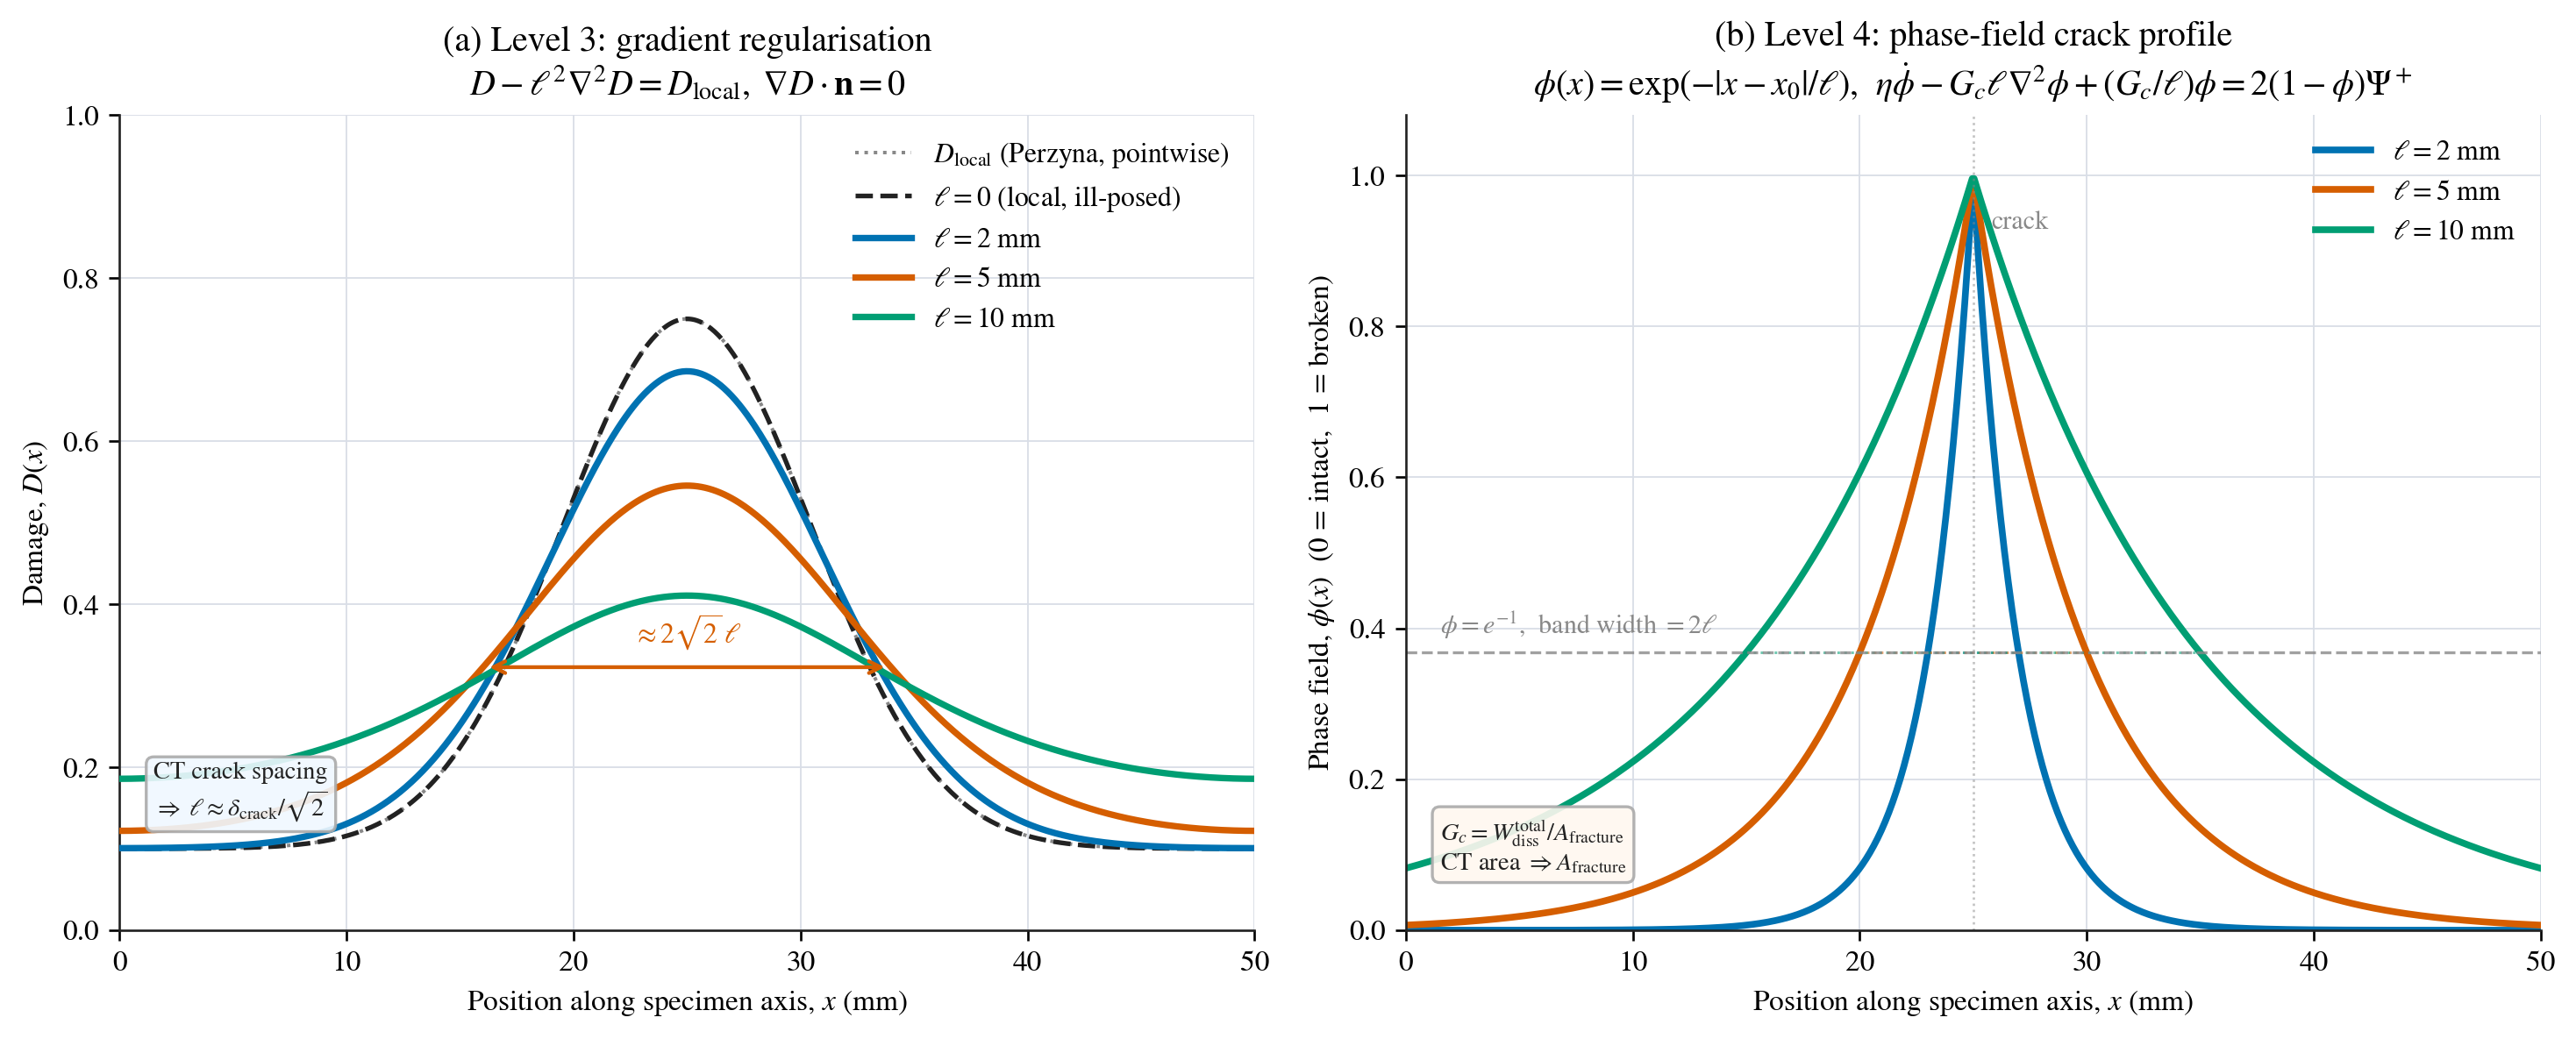
\includegraphics[width=\linewidth]{trihb_spatial_damage.png}
  \caption{Spatial damage verification for the Mode-3 Tri-HB reference case
  (specimen length $L=50$~mm, peak orthotropic damage $D_y\!\approx\!0.75$ from
  Fig.~\ref{fig:ortho}).
  (a)~Gradient regularisation (Eq.~\eqref{eq:gradD}): the pointwise Perzyna field
  $D_{\mathrm{local}}(x)$ (dotted) localises sharply for $\ell=0$ (dashed) and is
  smoothed into a finite process zone of width ${\approx}2\sqrt{2}\,\ell$ as $\ell$
  increases; $\ell$ is calibrated from the CT crack spacing $\delta_{\mathrm{crack}}$.
  (b)~Phase-field crack profile (Eq.~\eqref{eq:phicrack}): the equilibrium profile
  $\phi=\exp(-|x-x_0|/\ell)$ decays from unity at the crack centre; the band width
  $2\ell$ at the $e^{-1}$ level is directly measurable from CT cross-sections, and
  the Griffith energy follows from Eq.~\eqref{eq:gc} using the Step-3 dissipation,
  the CT fracture area, and an acoustic-emission or $K_{\mathrm{Ic}}$-based
  estimate of $\chi_f$.  Both models share the same $\ell$.}
  \label{fig:spatial}
\end{figure}

\section{Validation and calibration roadmap}\label{sec:roadmap}

The advances above are constitutive and computational; the system is presented
here as a measurement-and-modelling framework rather than a validated predictive
model. The decisive step is experimental: a staged, hierarchical calibration
that fixes the elastic and strength parameters before the damage kinetics, on a
\emph{calibration set} of tests, followed by \emph{blind prediction} on a disjoint
\emph{validation set}. The Tri-HB's unique strength is that its three independent
axes allow each anisotropic-damage component, each meridian of the failure
surface and each rate level to be probed directly. A practical matrix calibrates
the meridian and Lode parameters on a subset of confinements and strain rates and
blind-predicts held-out true-triaxial stress states ($\sigma_2\neq\sigma_3$),
while the directional damage components $D_x,D_y,D_z$ are
recovered post-test from per-axis ultrasonic modulus loss,
$D_i=1-E_{i,\mathrm{post}}/E_0$. Demonstrating that one calibrated parameter set
predicts strength and directional fracture on a held-out loading path is what
converts the framework from phenomenological to predictive, and is the natural
subject of the experimental campaign now enabled by the system.

\section{Conclusions}\label{sec:conclusion}

We have presented the Monash true-triaxial Hopkinson bar and its integrated
computational workspace. The six principal advances are: (i) a unified treatment of
uniaxial, axisymmetric-confined and true-triaxial static--dynamic loading as
special cases of a single gas-gun system; (ii) a true-triaxial, Lode-angle- and rate-dependent failure
envelope that captures the intermediate principal stress effect with the correct
sign; (iii) an energy-consistent damage--dissipation partition in which the first
law closes by construction with non-negative dissipation; (iv) an orthotropic damage tensor whose
directional components reproduce the oriented fracture of rock blasting and can be
calibrated component-by-component from the system's direction-resolved
measurements; (v) a cumulative-damage model for repeated (cyclic) dynamic
loading that captures the sudden, few-impact dynamic-fatigue failure of a
pre-stressed rock mass; and (vi) a spatial thermodynamic extension --- a
gradient-regularised damage field (internal length $\ell$ from CT crack spacing,
Eq.~\eqref{eq:gradD}) and a phase-field formulation (Griffith energy $G_c$ from
the measured dissipation and CT fracture area, Eq.~\eqref{eq:gc}; crack profile
validated against CT attenuation maps, Eq.~\eqref{eq:phicrack}) that is
thermodynamically consistent by construction and directly comparable to
post-impact CT cross-sections from the Tri-HB campaign.  Together, the hardware
and its computational workspace establish a platform for quantitative, multiaxial
dynamic constitutive modelling of rock; the immediate next step is the experimental
calibrate-then-blind-predict campaign that the system uniquely enables.

\backmatter

\bmhead{Declarations}
\noindent\textbf{Funding.} Not declared (development study).\\[2pt]
\textbf{Competing interests.} The author declares no competing interests.\\[2pt]
\textbf{Data and code availability.} The Virtual Tri-HB workspace
(\texttt{tri\_hb\_integrated.py}) and the figure-generation scripts used here are
part of the Tri-HB repository. All figures in this paper are produced from
prescribed-pulse reference cases by the workspace's own analysis pipeline; no
experimental data were used.\\[2pt]
\textbf{Author contributions.} Q.B.Z. conceived the system and the workspace
framework, implemented the analysis pipeline, and wrote the manuscript.

\bibliography{refs}

\end{document}
